\subsection{Overview}
This section is intended to explain in detail all the components used by the system in order to offer all the functionalities.\\
The figure \ref{fig:hilvl} below shows the high-level architecture of the system-to-be. All the components are better explained in the following paragraphs.\\
\begin{figure}[h]
    \centering
    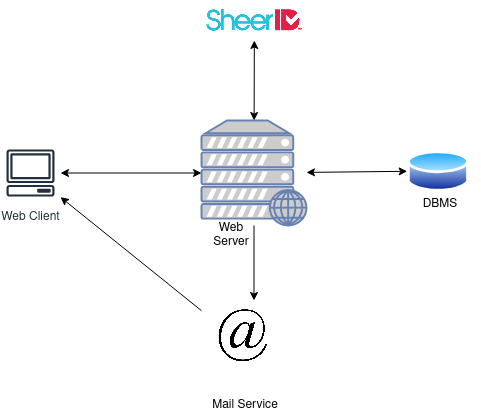
\includegraphics[width=1\linewidth]{Images/S&C_DD-High Level System Overview.drawio.png}
    \caption{High level architecture}
    \label{fig:hilvl}
\end{figure}

\subsection{Component view}
The Students\&Companies platform will be implemented using a three tier architecture. Figure \ref{fig:compview} shows the component view diagram of the platform. The WebApp (presentation layer) will use functions implemented in the business layer through API calls. The business layer interacts with SheerID for the student login functionality.\\
\begin{figure}[h]
    \centering
    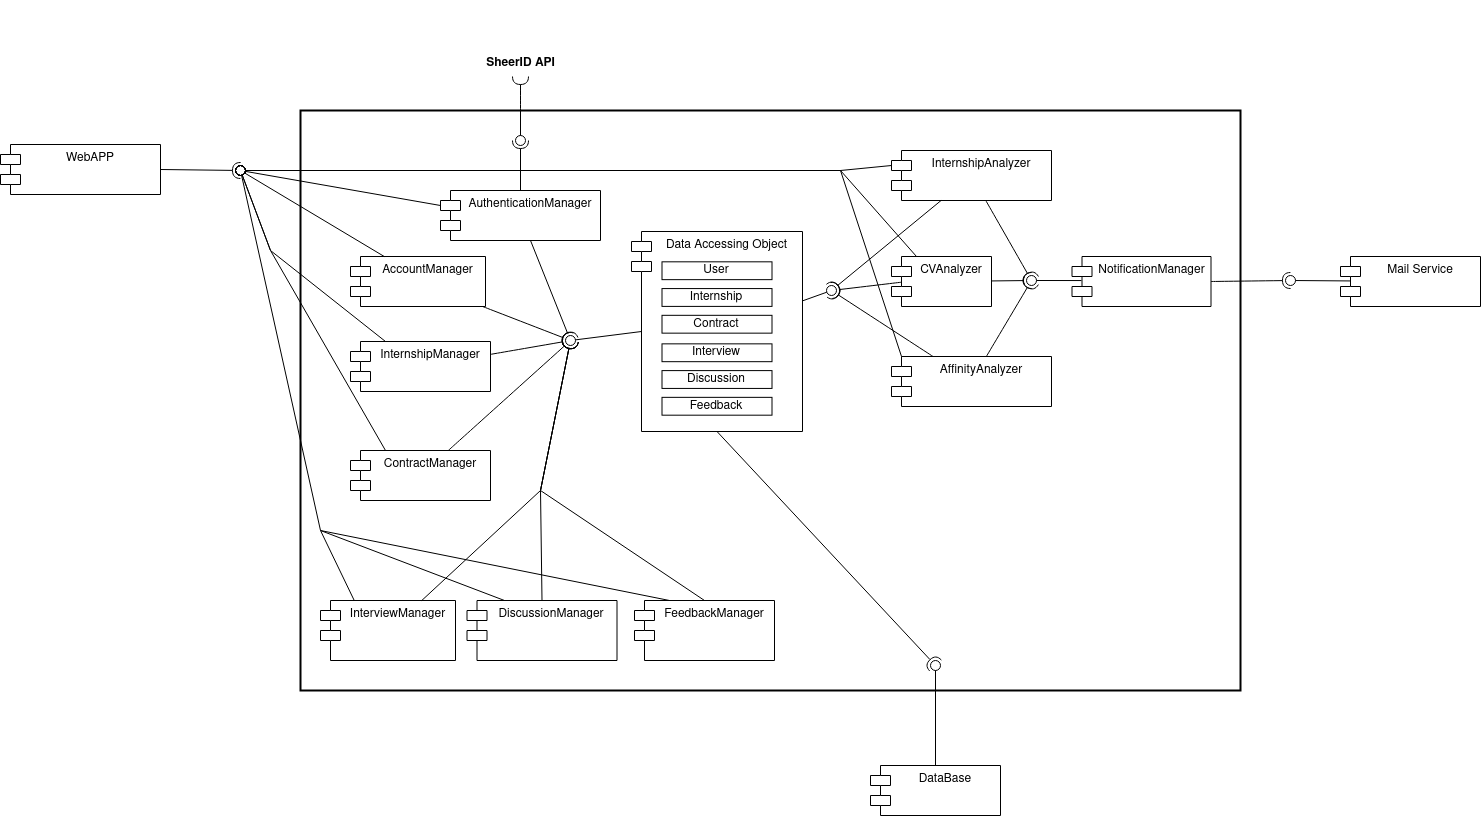
\includegraphics[width=1\linewidth]{Images/comp_view.png}
    \caption{Component view of the system}
    \label{fig:compview}
\end{figure}\\
The system is comprised of the following components:
\begin{itemize}
    \item \textbf{Data Accessing Object (DAO)}: a set of classes utilized to interact with the database, facilitating the retrieval and uploading of information. This approach ensures a single component manages the database connection and handles the query language.
    \item \textbf{AuthenticationManager}: component used for managing user’s registration and login. It uses DAO’s interfaces to manage companies and universities information and SheerID’s API to manage students’ login.
    \item \textbf{AccountManager}: component used to allow the user to modify his profile.
    \item \textbf{InternshipManager}: component used to help users to manage internships.
    \item \textbf{ContractManager}: component used to help users to manage contract stipulations.
    \item \textbf{InterviewManager}: component used to help users to manage interviews.
    \item \textbf{DiscussionManager}: component used to help users to manage discussions.
    \item \textbf{FeedbackManager}: component used to help users to manage feedback.
    \item \textbf{InternshipAnalyzer}: component that produces analytics on internship descriptions based on info collected from the database through DAOs. It relies on the NotificationManager to send notifications to final users.
    \item \textbf{CVAnalyzer}: component that produces analytics on CVs based on info collected from the database through DAOs. It relies on the NotificationManager to send notifications to final users.
    \item \textbf{AffinityAnalyzer}: component that produces analytics on CVs and internship positions based on info collected from the database through DAOs. It relies on the NotificationManager to send notifications to final users.
    \item \textbf{NotificationManager}: component used to abstract the service used to send notifications from the other components.
\end{itemize}

\subsection{Deployment view}
The organization of S\&C's physical infrastructure is shown in figure \ref{fig:deployment}. As it is possible to see, the system uses a single server to host the database, while an array of replicated servers runs the components related to the buisness logic.\\
\begin{figure}[h]
    \centering
    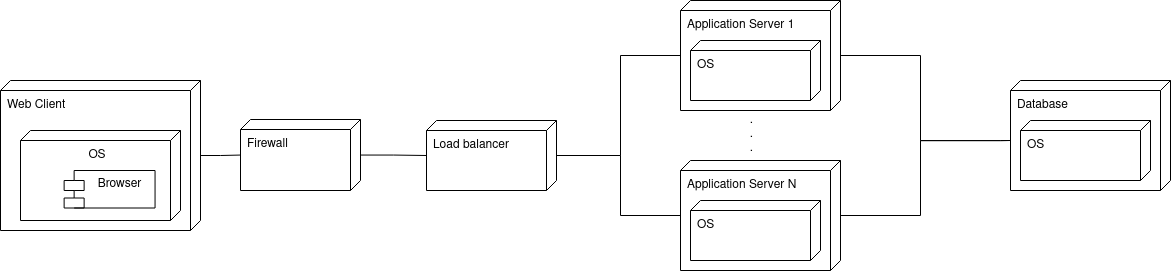
\includegraphics[width=1\linewidth]{Images/deployment.png}
    \caption{Deployment view}
    \label{fig:deployment}
\end{figure}\\
In more detail, the system architecture is made of:
\begin{itemize}
    \item \textbf{WebClient}: the user's device, running a browser which is used to interact with the system.
    \item  \textbf{Firewall}: a firewall to protect the system from potential malicious attacks.
    \item \textbf{Load balancer}: a component used to distribute incoming requests to different replicated servers based on individual loads.
    \item \textbf{Application server}: the server in charge of handling requests from the clients. To ensure acceptable performance even under high loads this server is replicated.
    \item \textbf{Database}: a server dedicated to run the DBMS.
\end{itemize}





\subsection{Runtime View}
[UC1] - Company Registration\newline
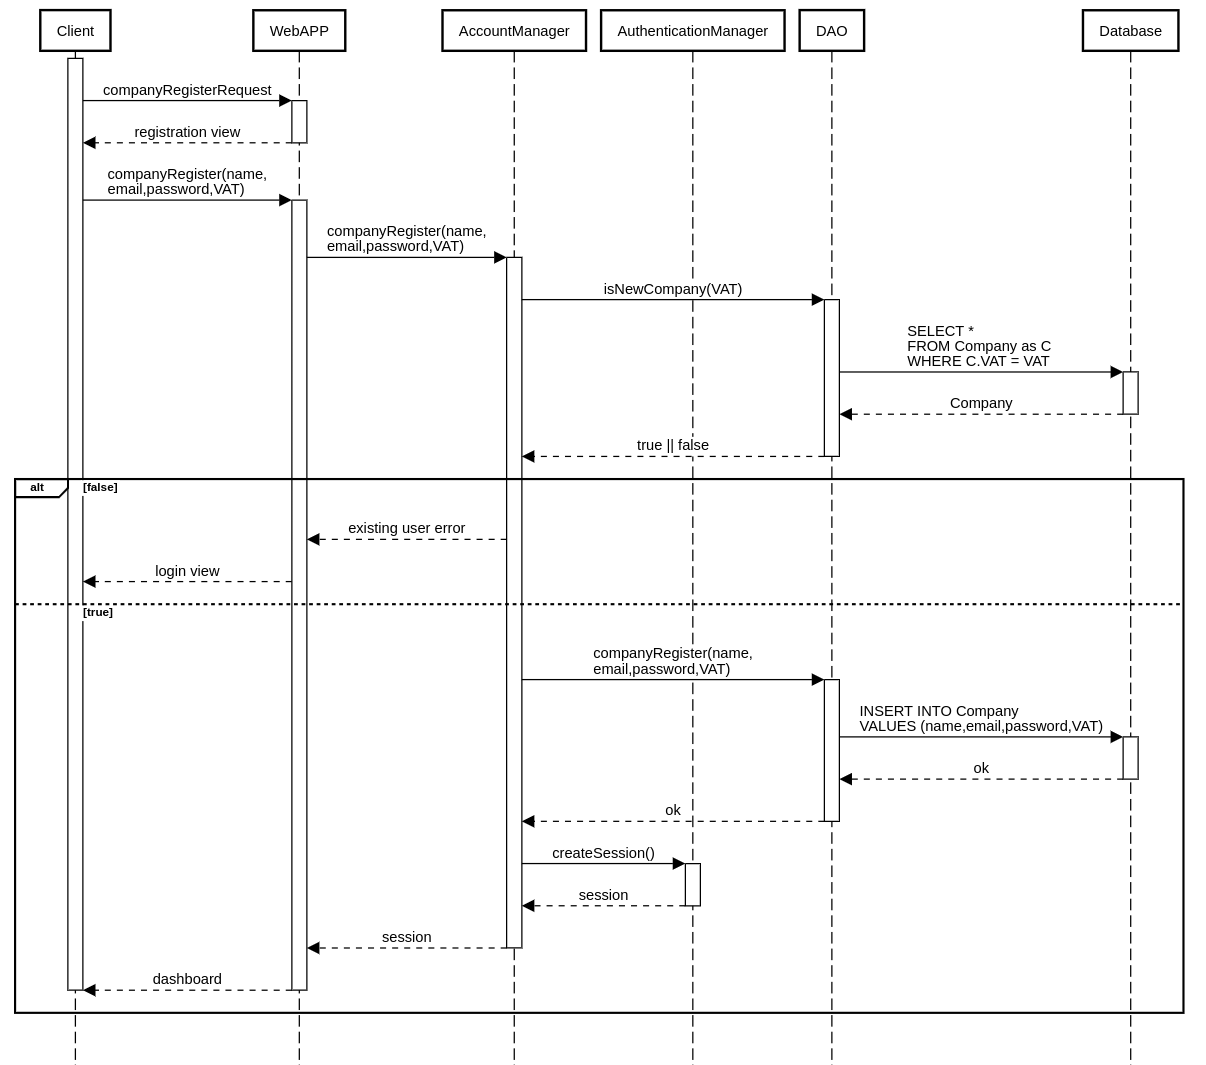
\includegraphics[width=\textwidth]{Images/UC diagrams/company_registration.png}\newpage
[UC2] - Company Login\newline
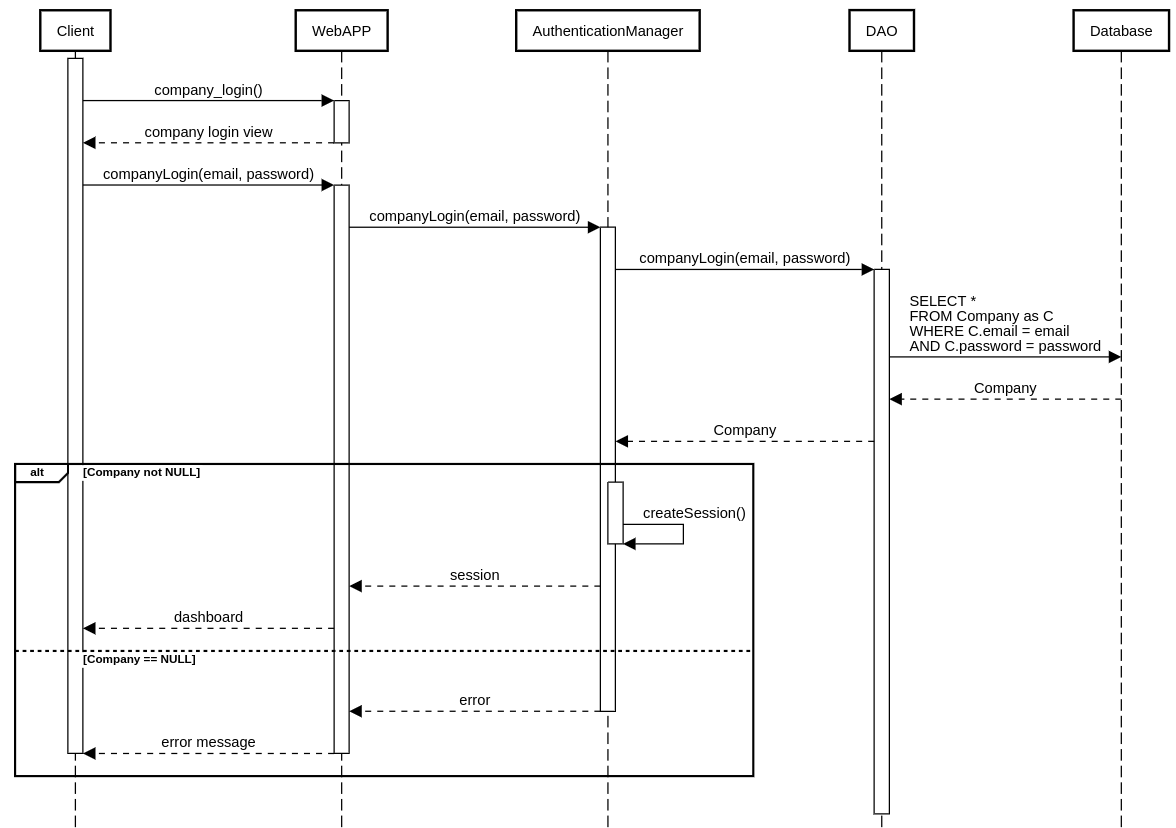
\includegraphics[width=\textwidth]{Images/UC diagrams/company_login.png}\newline
[UC3] - University Login\newline
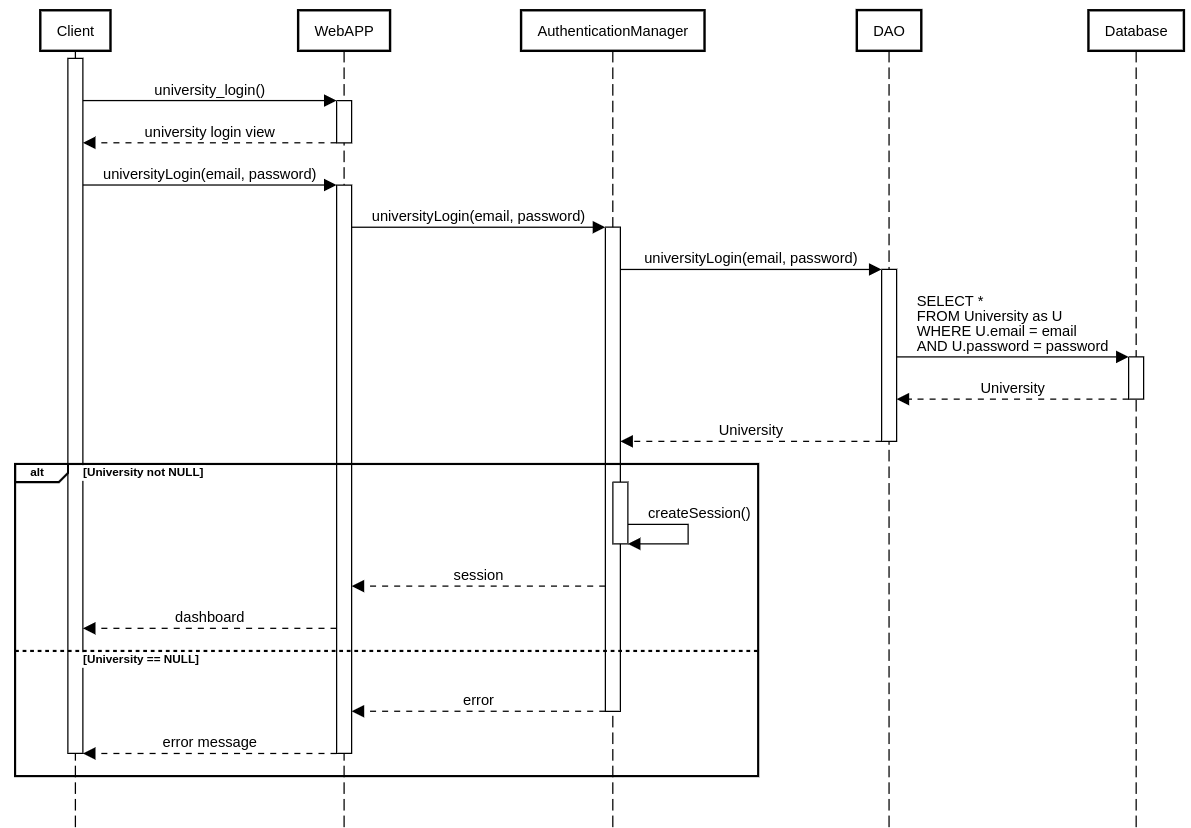
\includegraphics[width=\textwidth]{Images/UC diagrams/university_login.png}\newpage
[UC4] - Student Login\newline
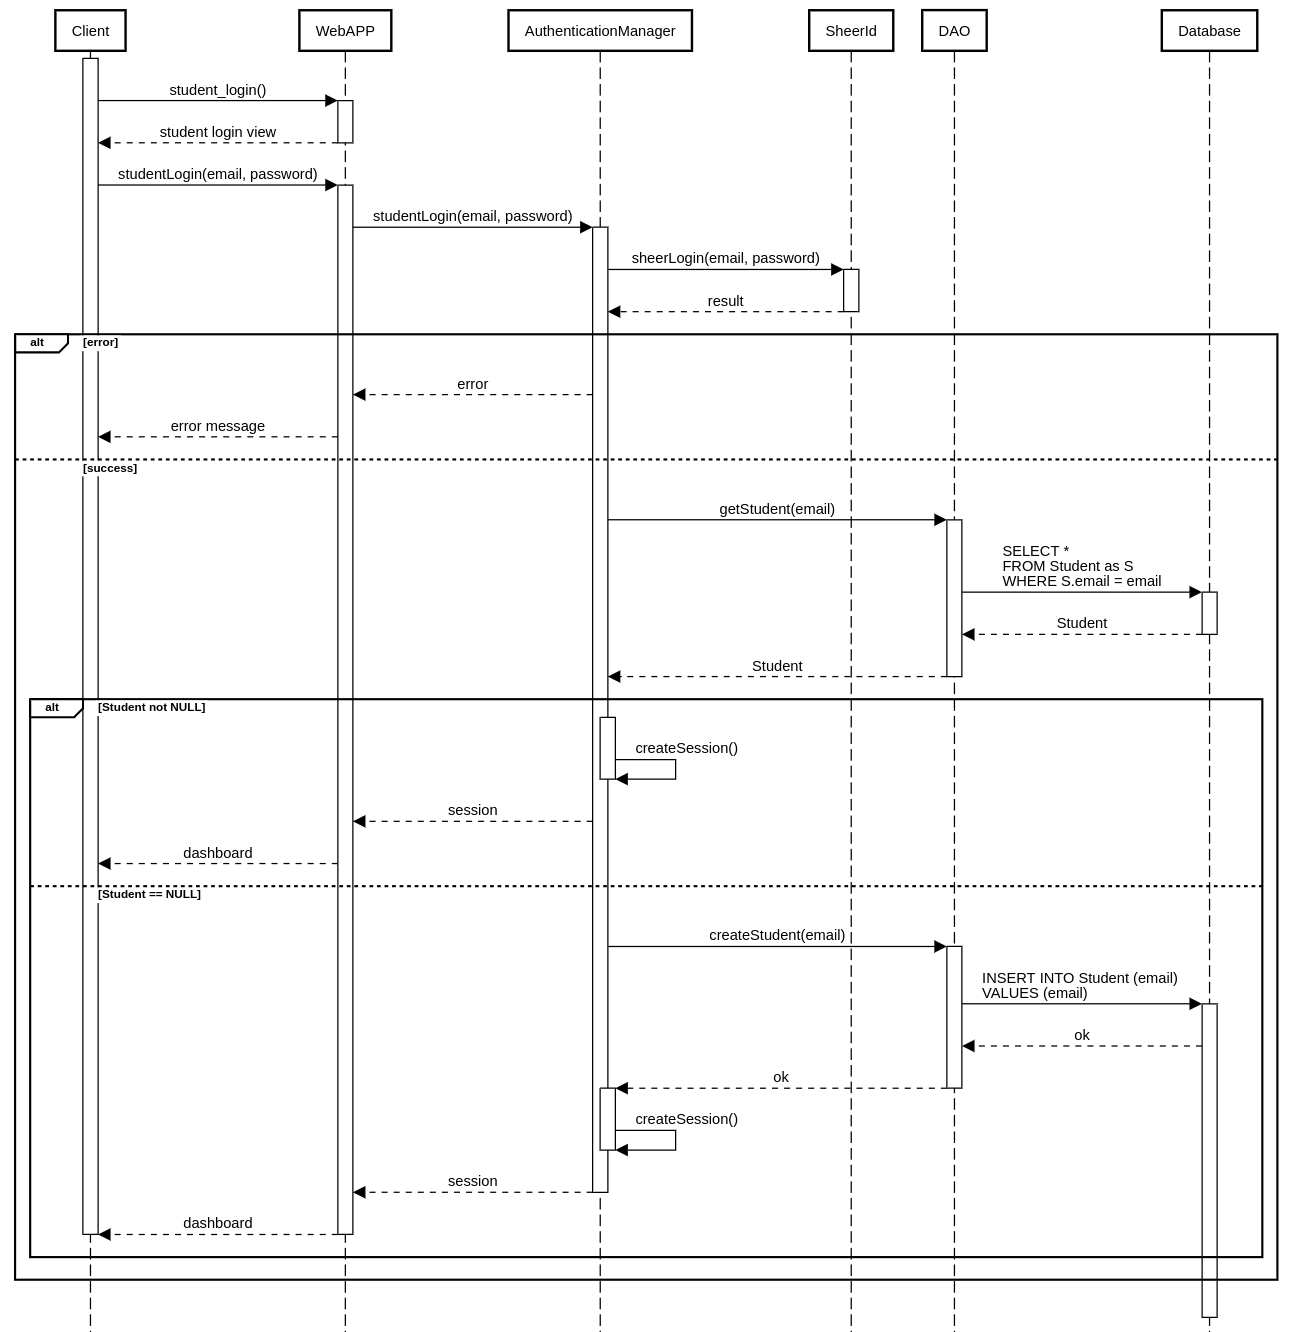
\includegraphics[width=\textwidth]{Images/UC diagrams/student_login.png}\newpage
[UC5] - Post Internship\newline
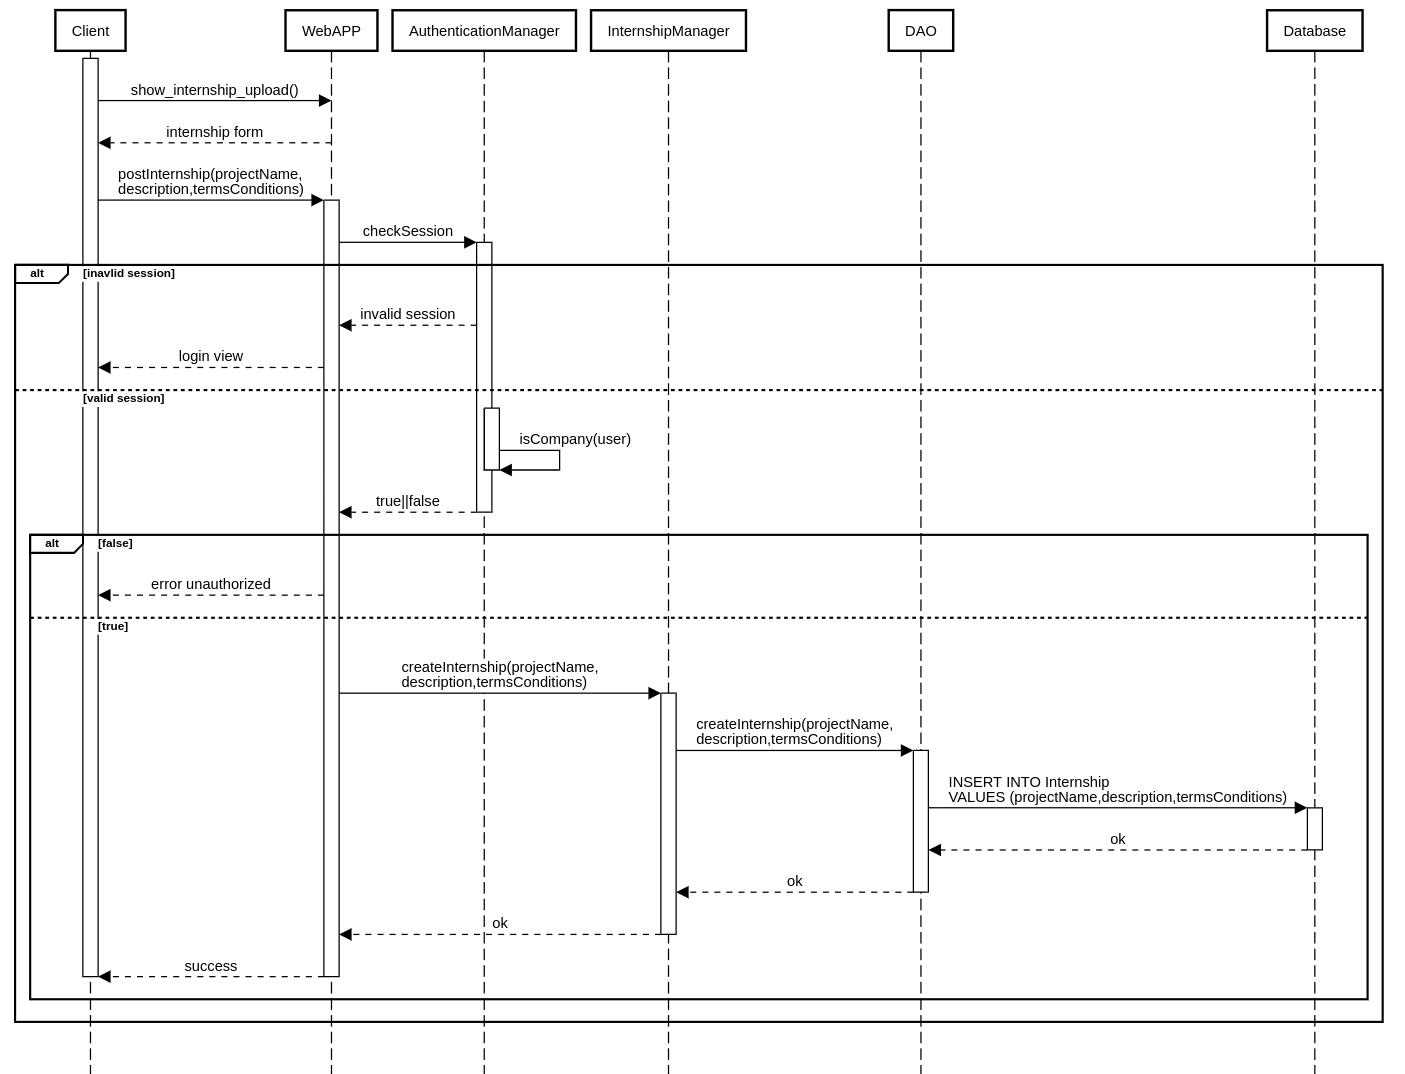
\includegraphics[width=\textwidth]{Images/UC diagrams/post_internship.png}\newpage
[UC6] - Post Feedback\newline
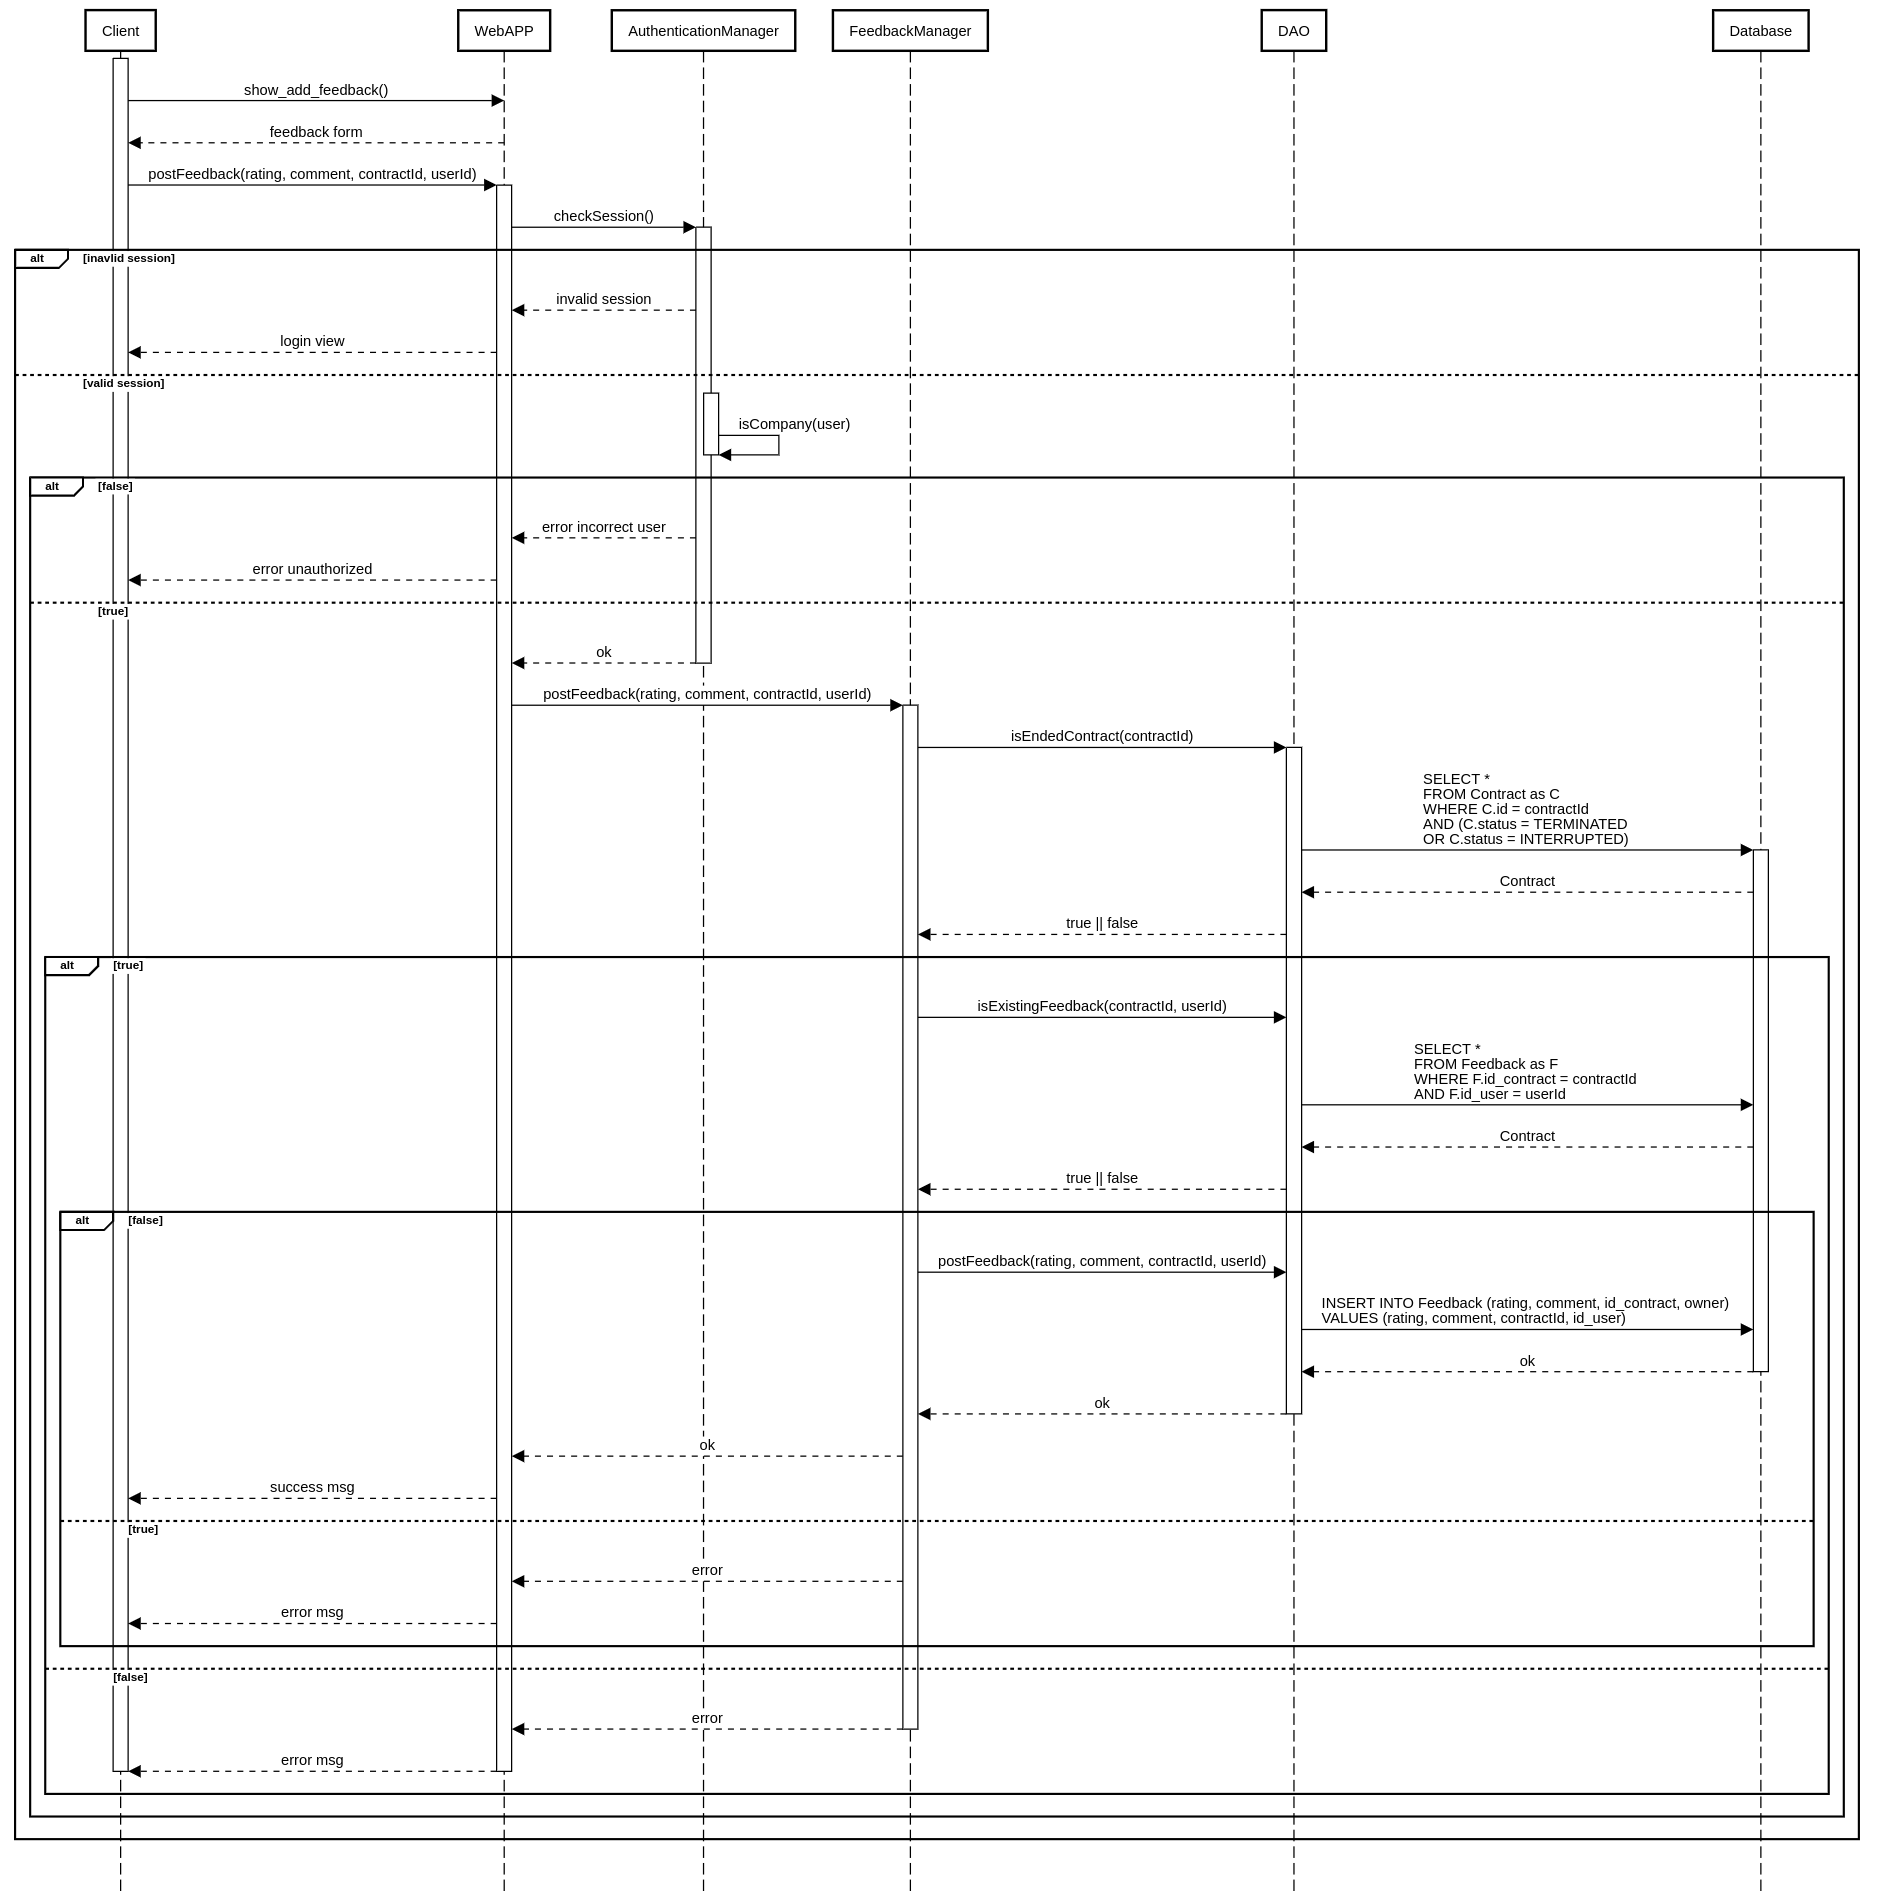
\includegraphics[width=\textwidth]{Images/UC diagrams/post_feedback.png}\newpage
[UC7] - Search Internship\newline
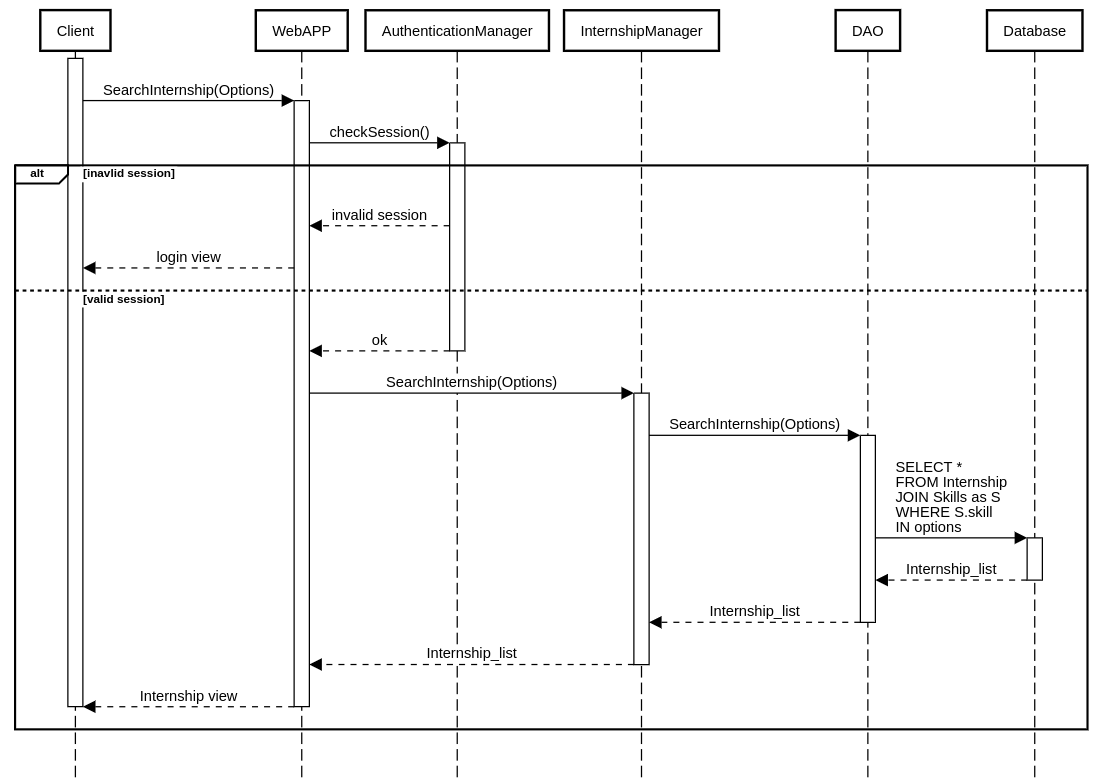
\includegraphics[width=\textwidth]{Images/UC diagrams/search_internship.png}\newpage
[UC8] - Apply for an Internship\newline
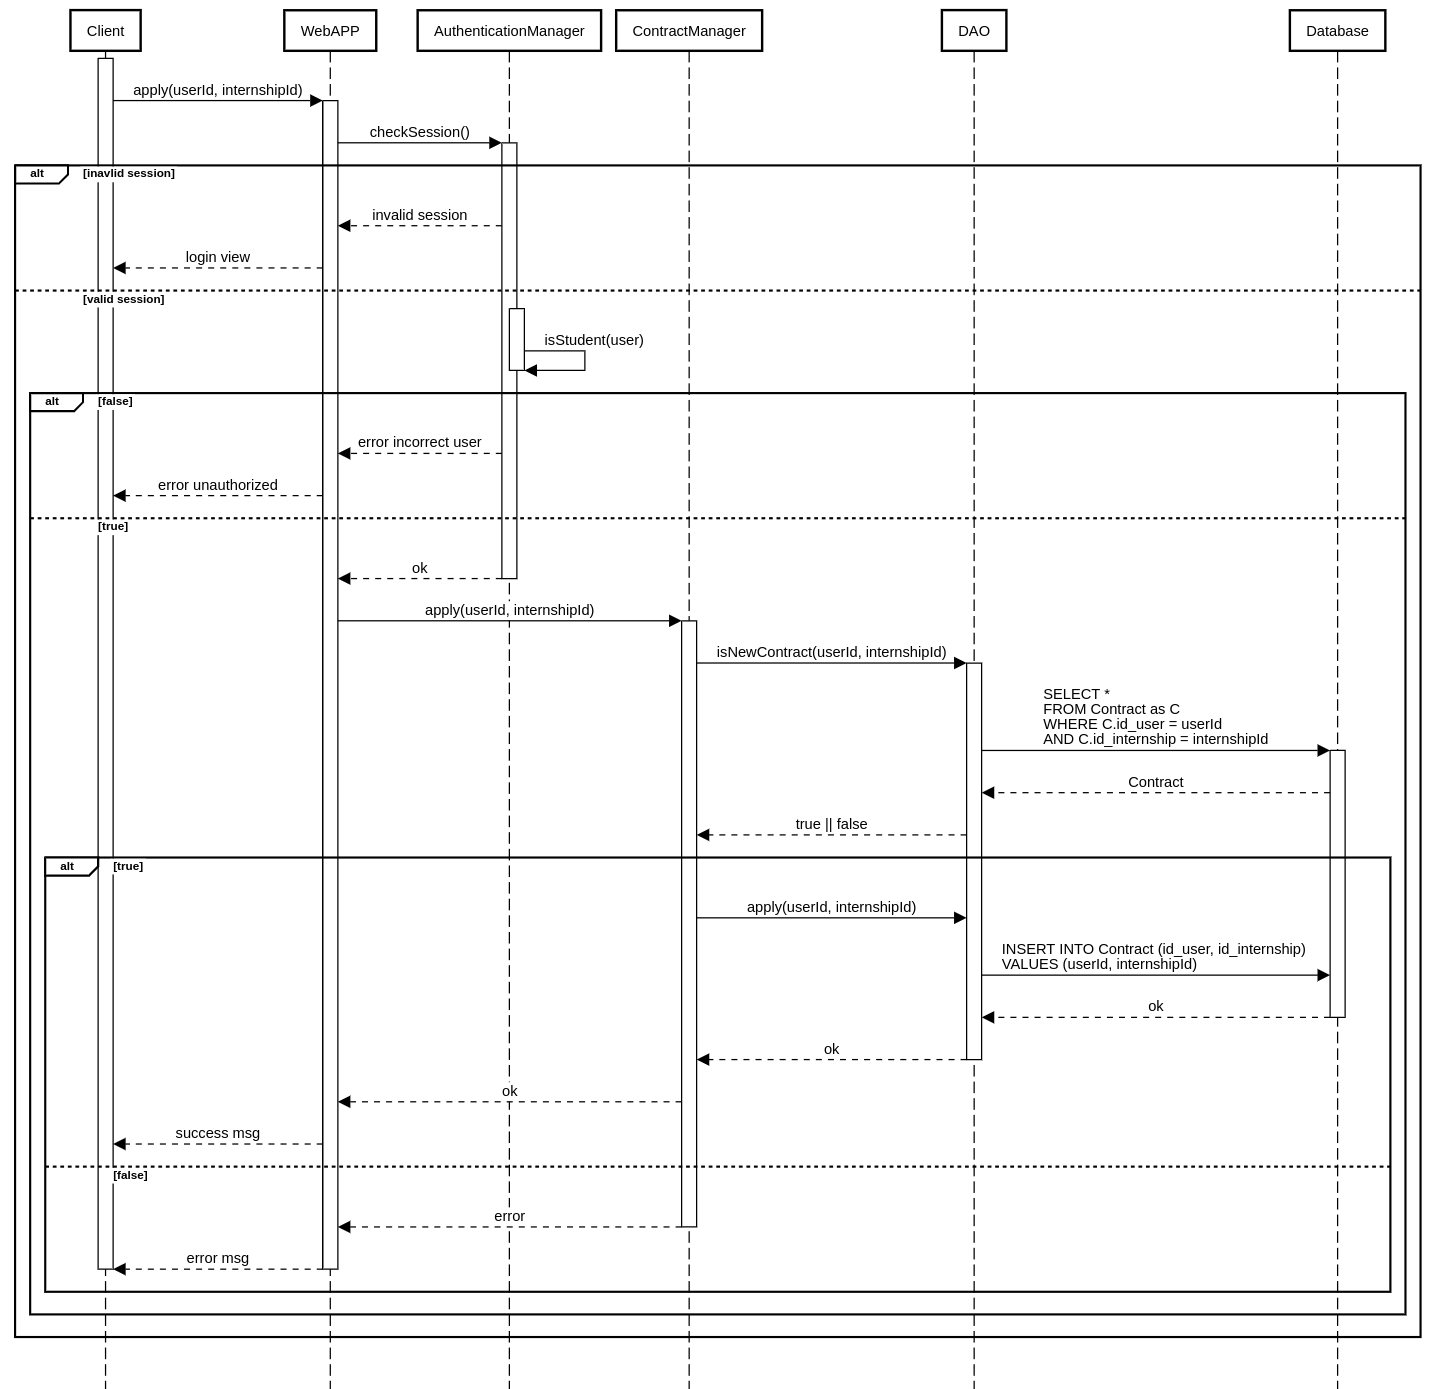
\includegraphics[width=\textwidth]{Images/UC diagrams/apply_internship.png}\newpage
[UC9] - Questionnaire Creation\newline
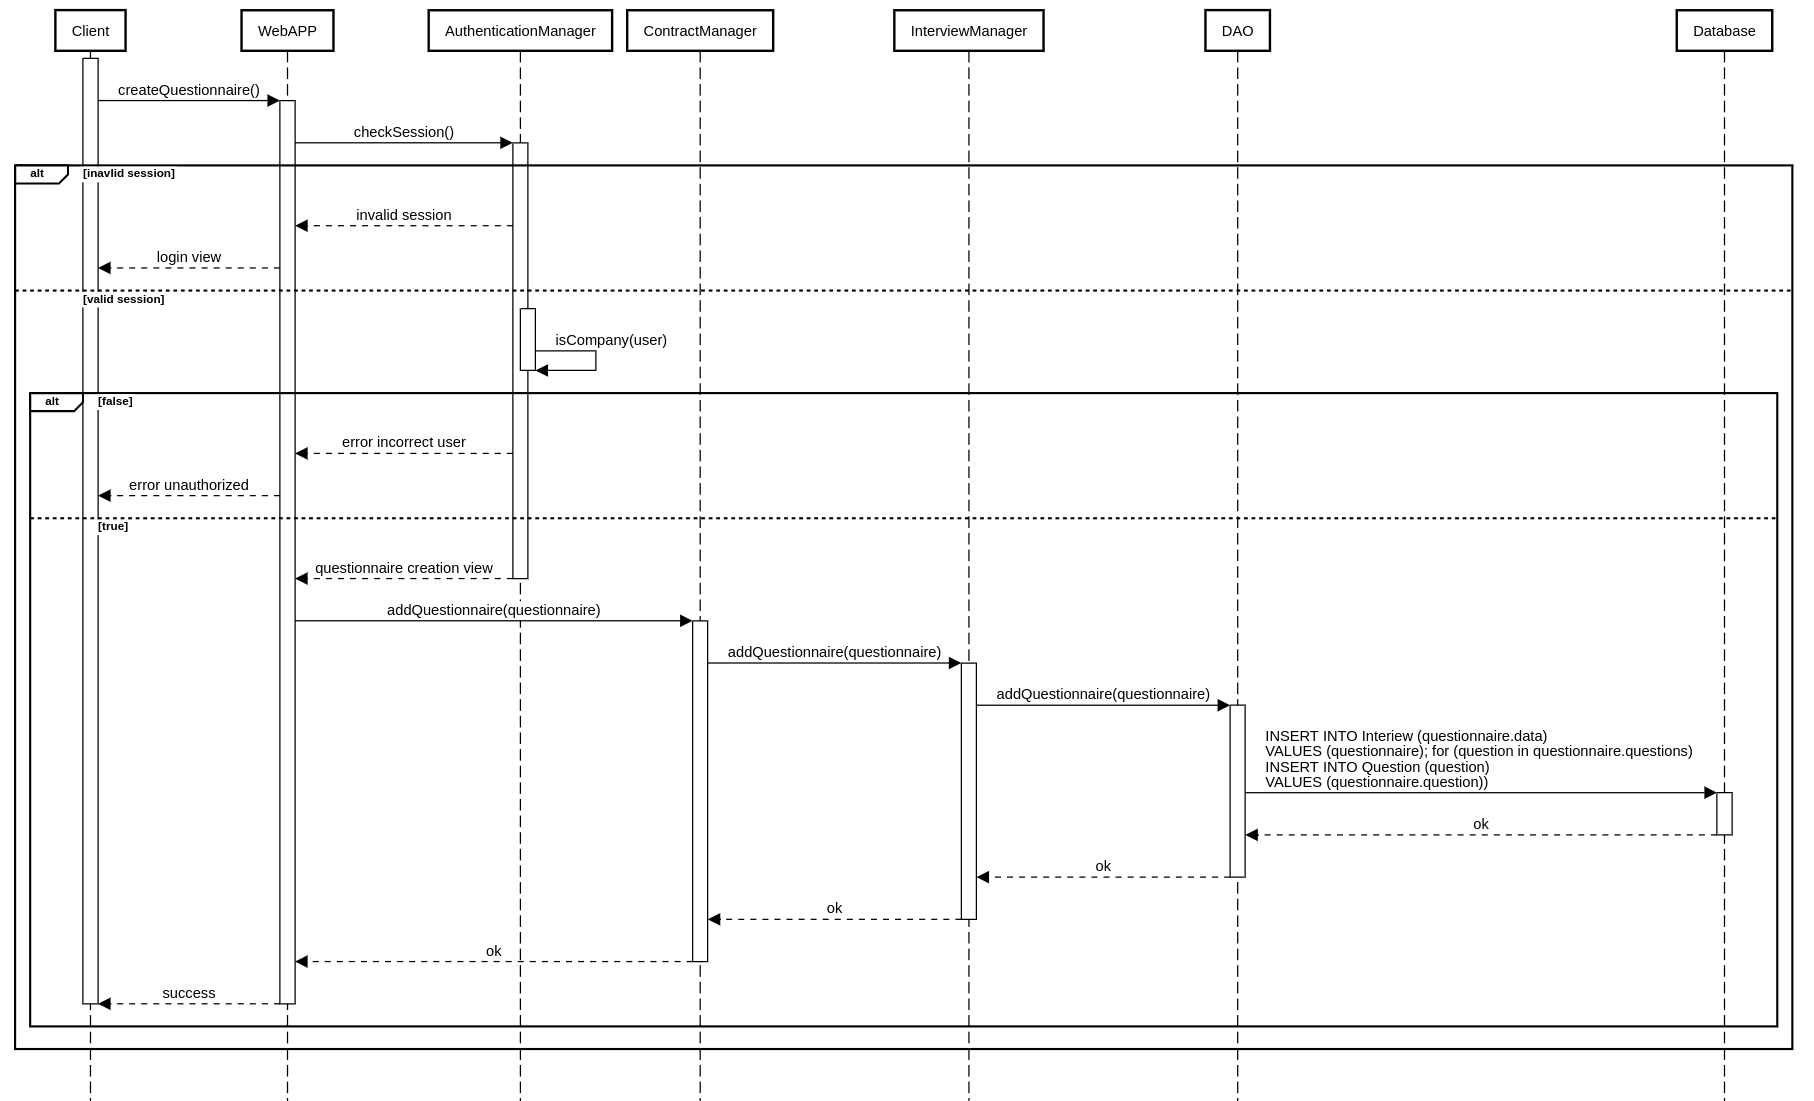
\includegraphics[width=\textwidth]{Images/UC diagrams/questionnaire_creation.png}\newpage
[UC10] - Answer Questionnaire Interview\newline
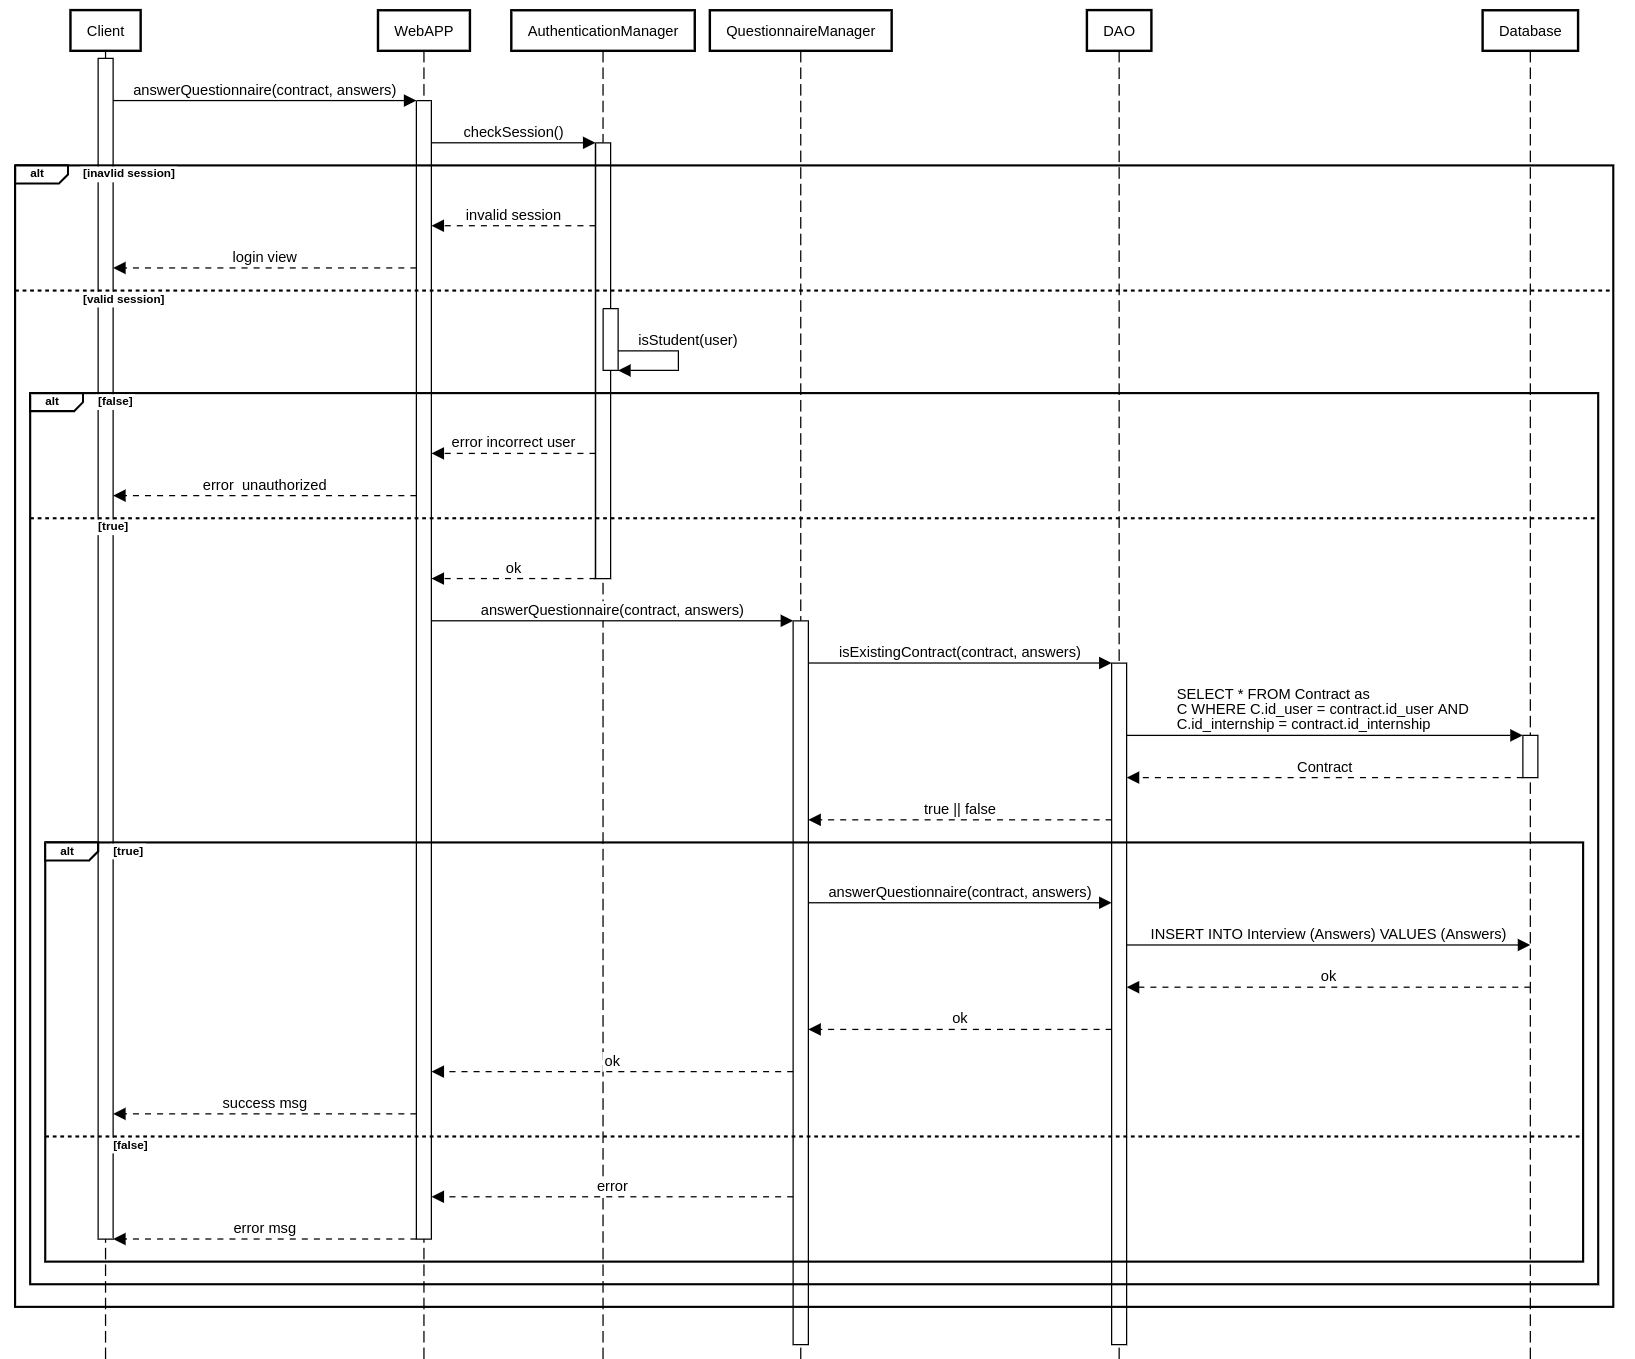
\includegraphics[width=\textwidth]{Images/UC diagrams/answer_questionnaire.png}\newpage
[UC11] - Sign Contract\newline
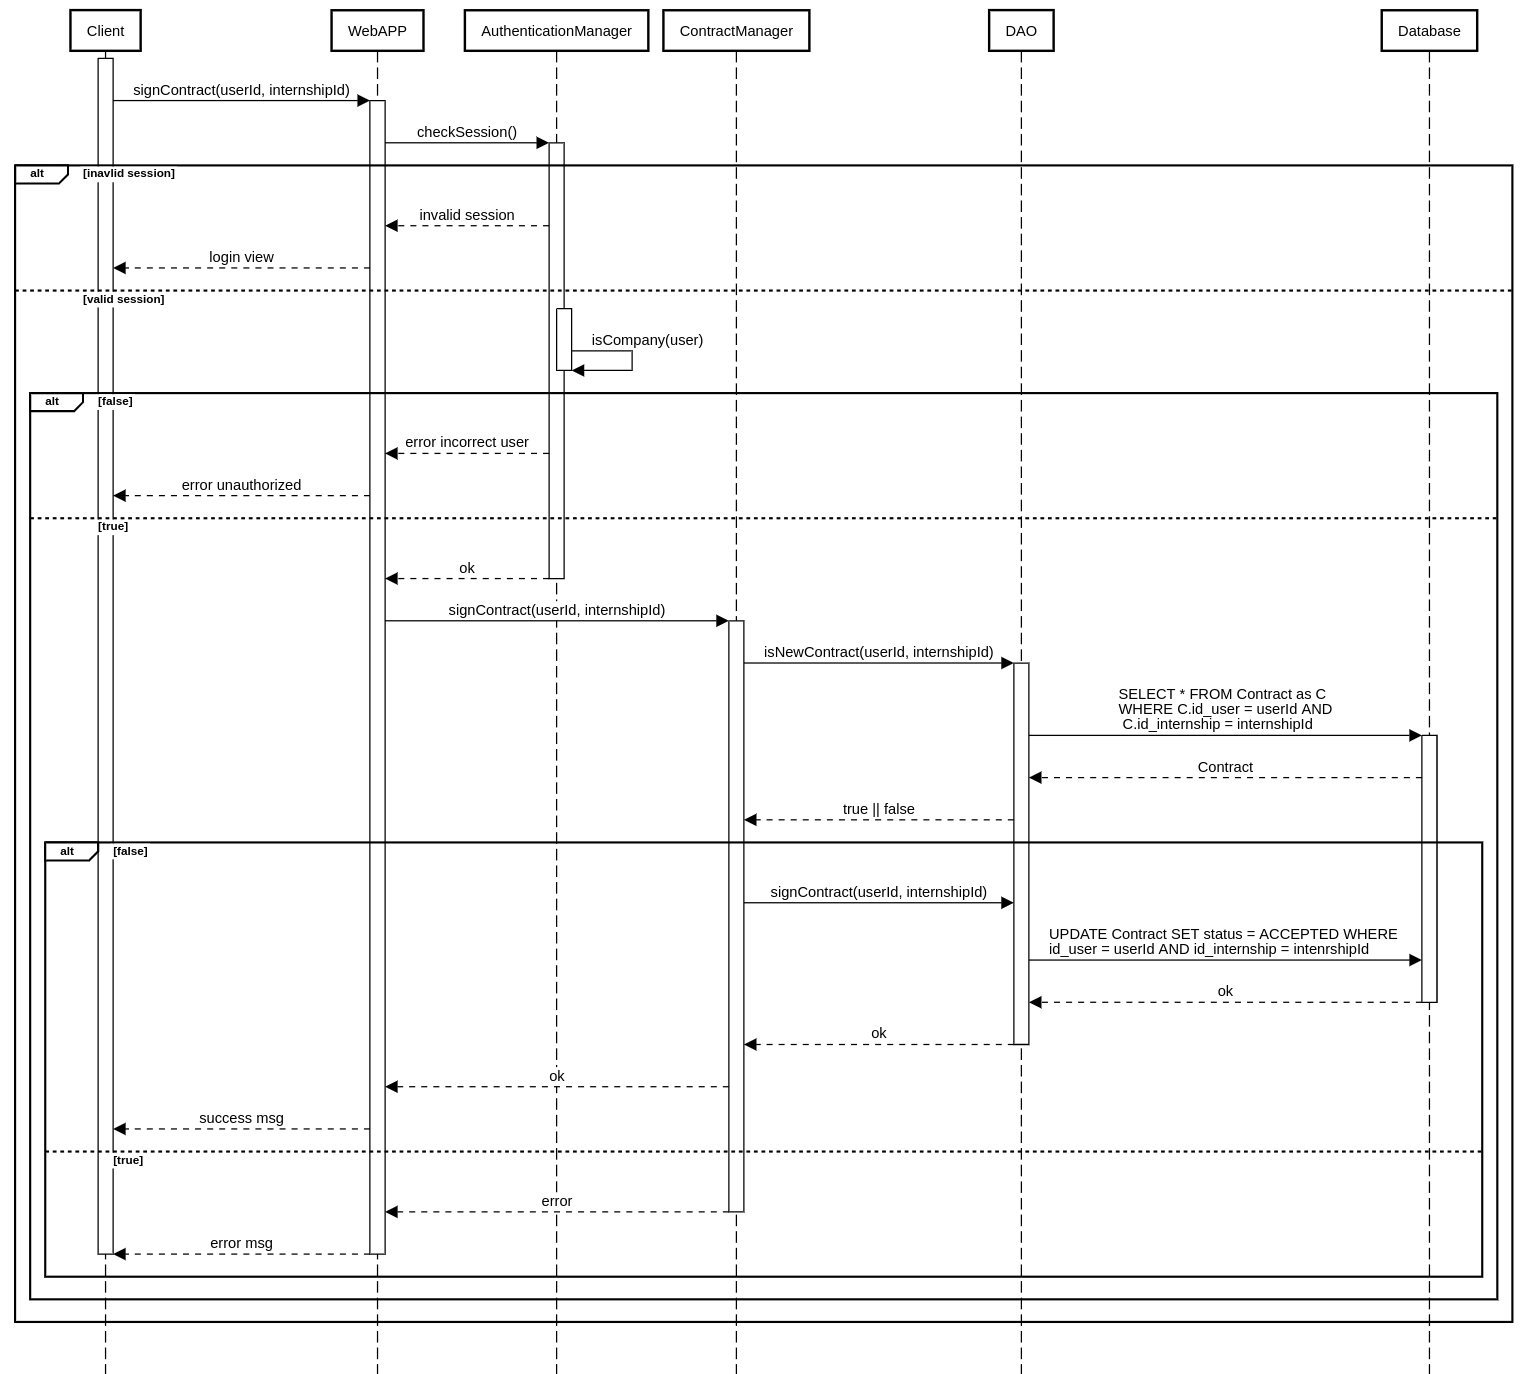
\includegraphics[width=\textwidth]{Images/UC diagrams/sign_contract.png}\newpage
[UC12] - Open Discussion\newline
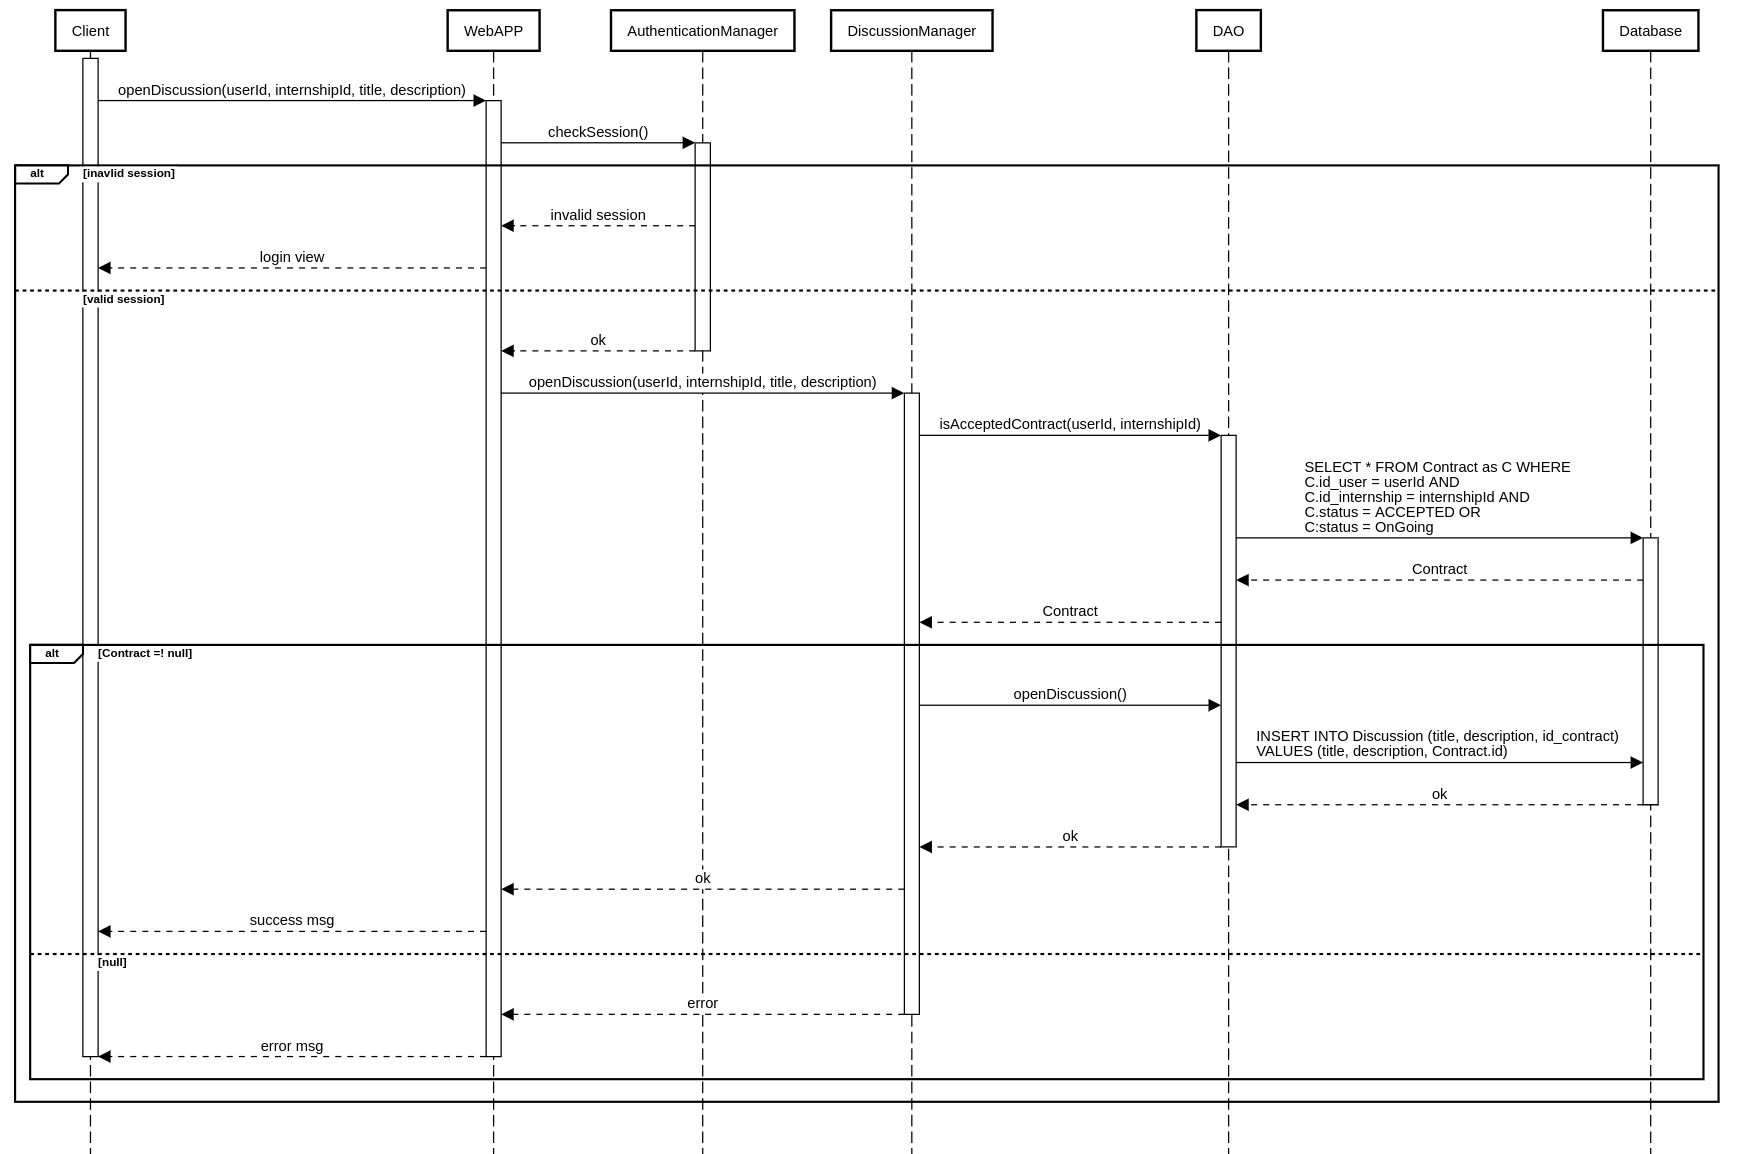
\includegraphics[width=\textwidth]{Images/UC diagrams/open_discussion.png}\newline
[UC13] - Send Message in a Discussion\newline
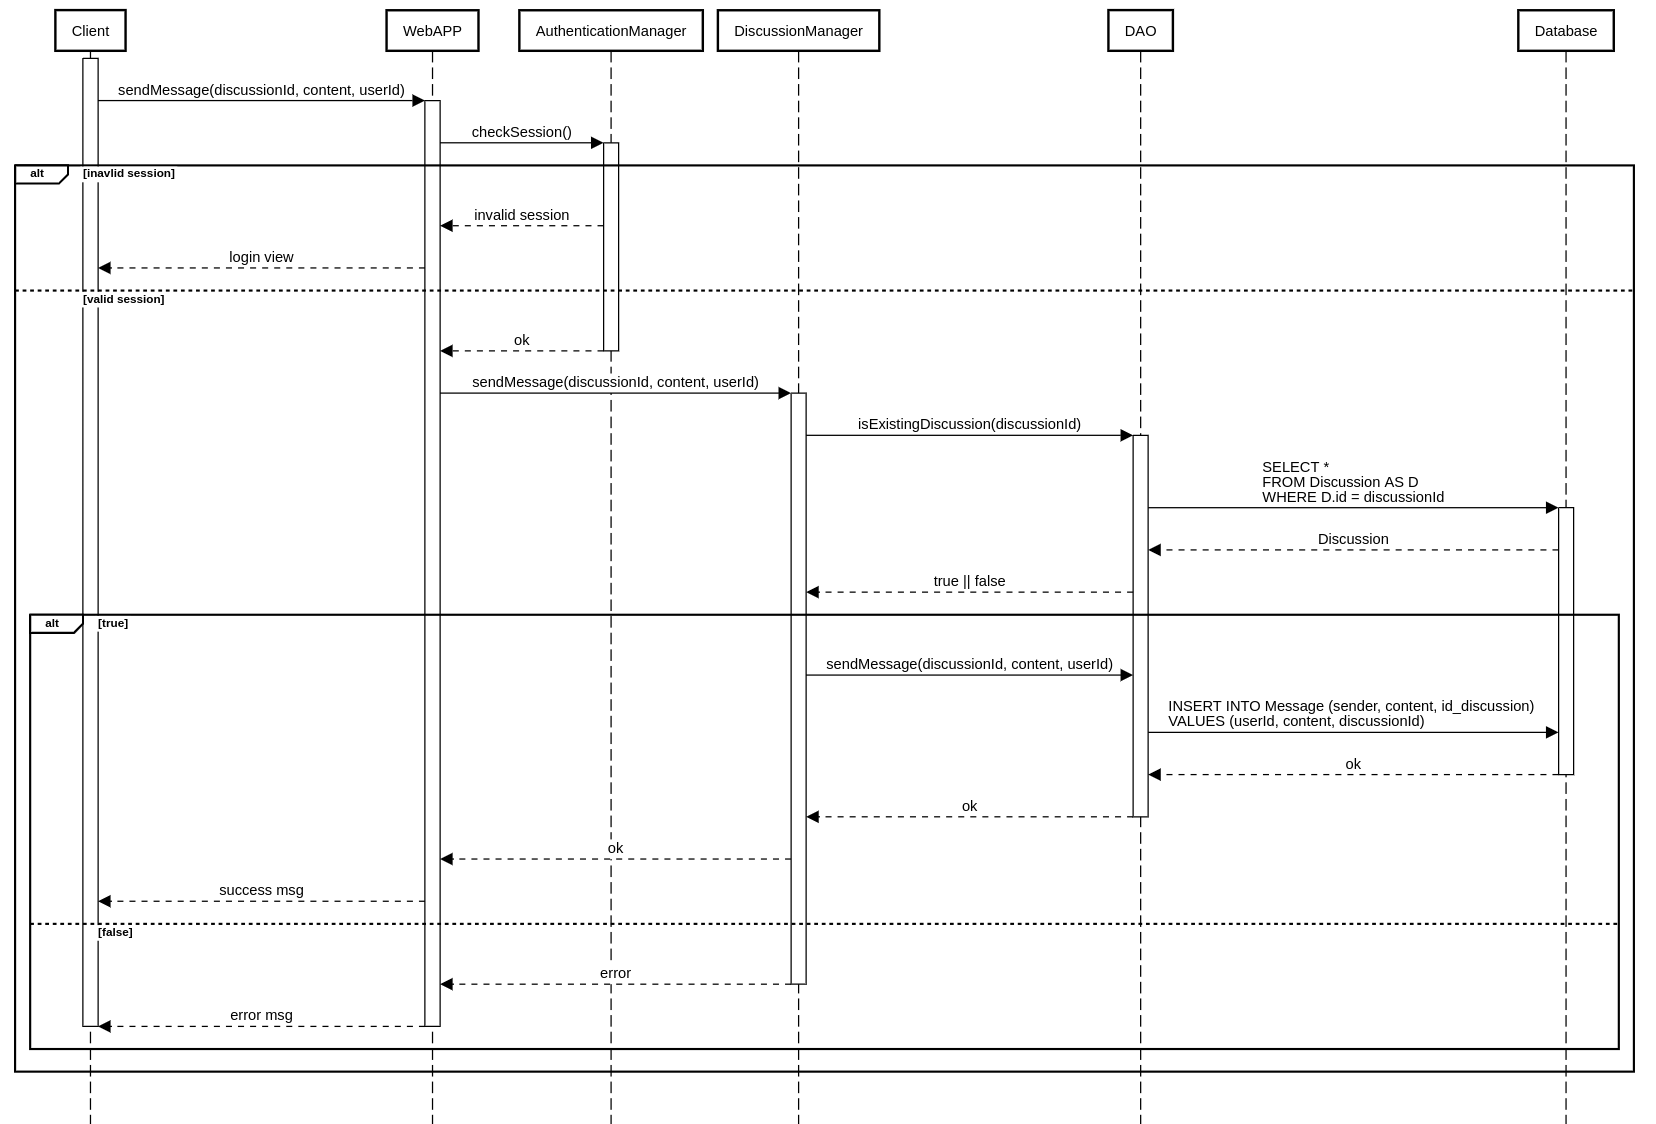
\includegraphics[width=\textwidth]{Images/UC diagrams/send_message.png}\newpage
[UC14] - Terminate Internship\newline
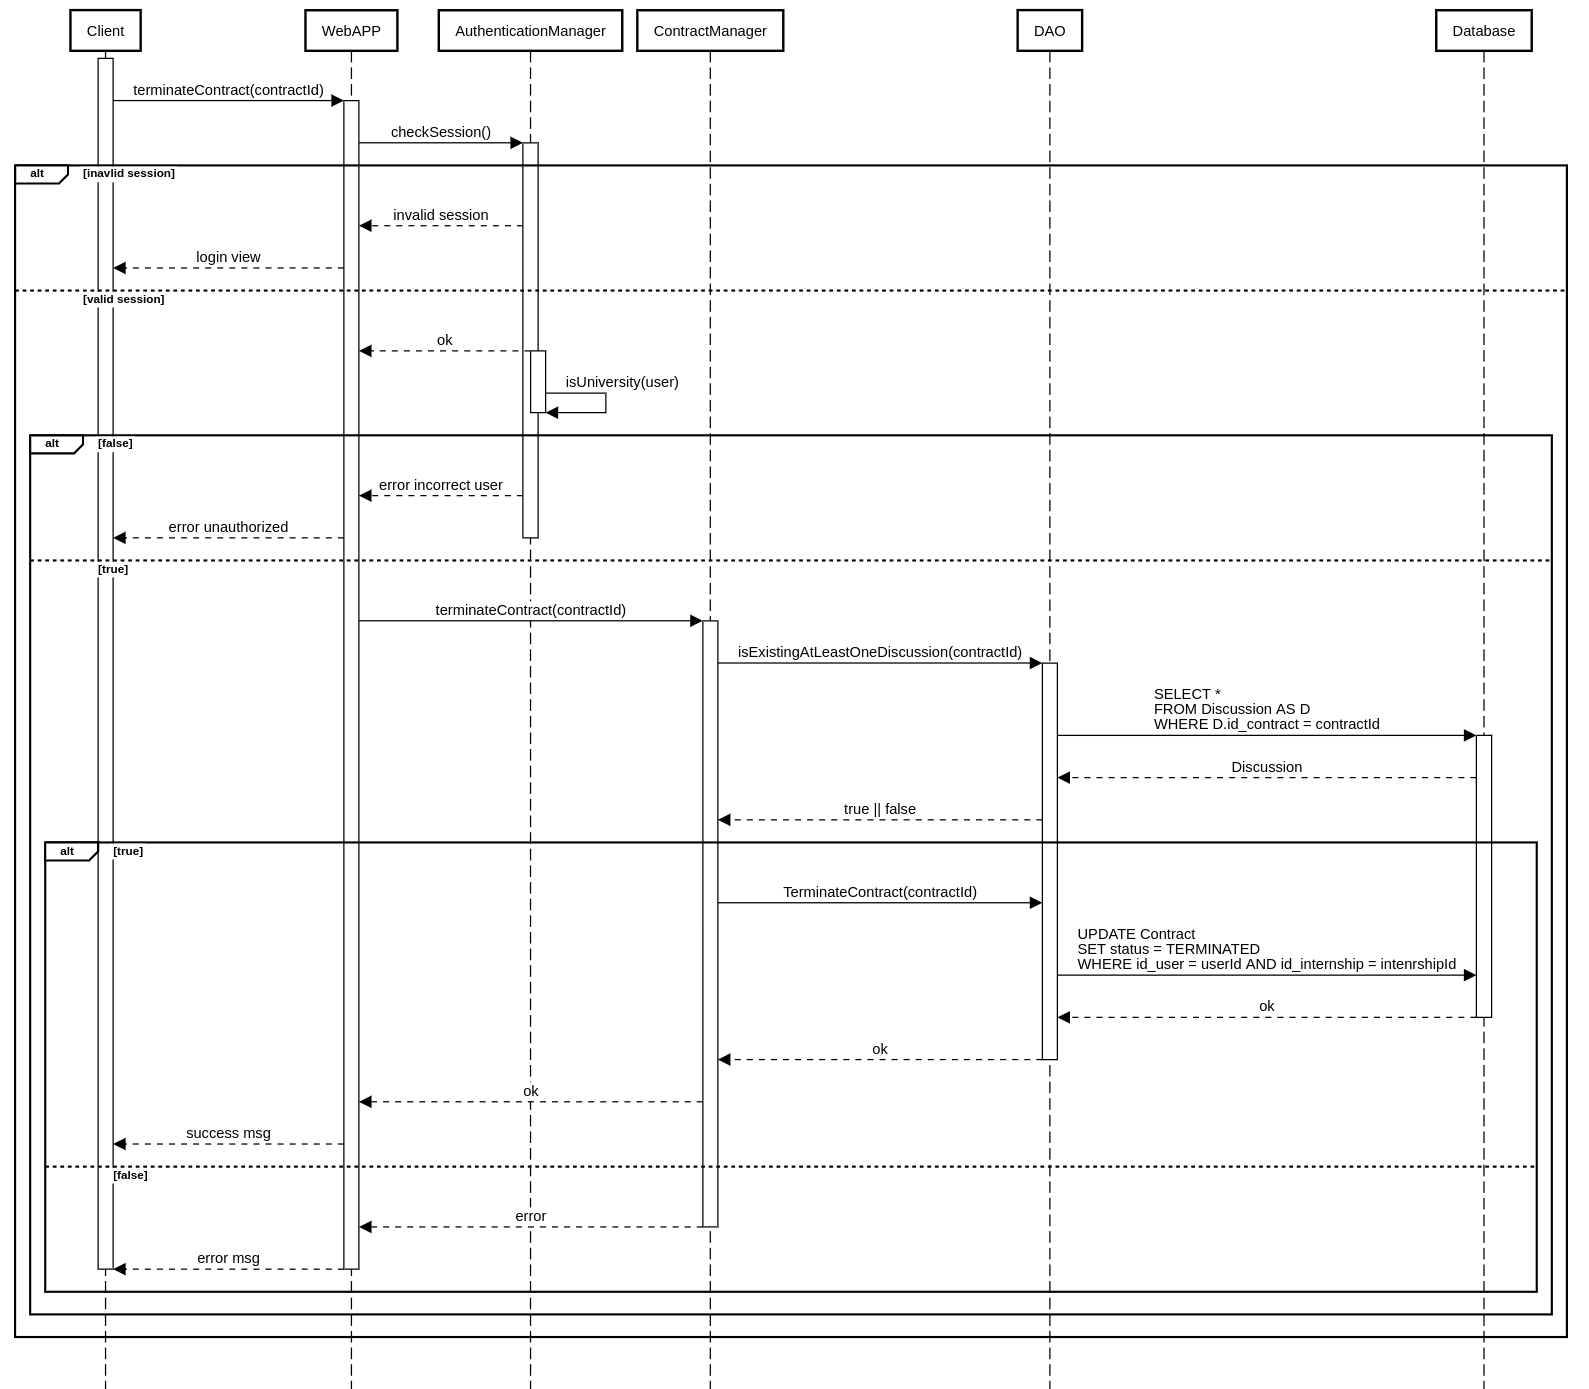
\includegraphics[width=\textwidth]{Images/UC diagrams/terminate_internship.png}\newline
[UC15] - Generate CV Improvement Suggestion\newline
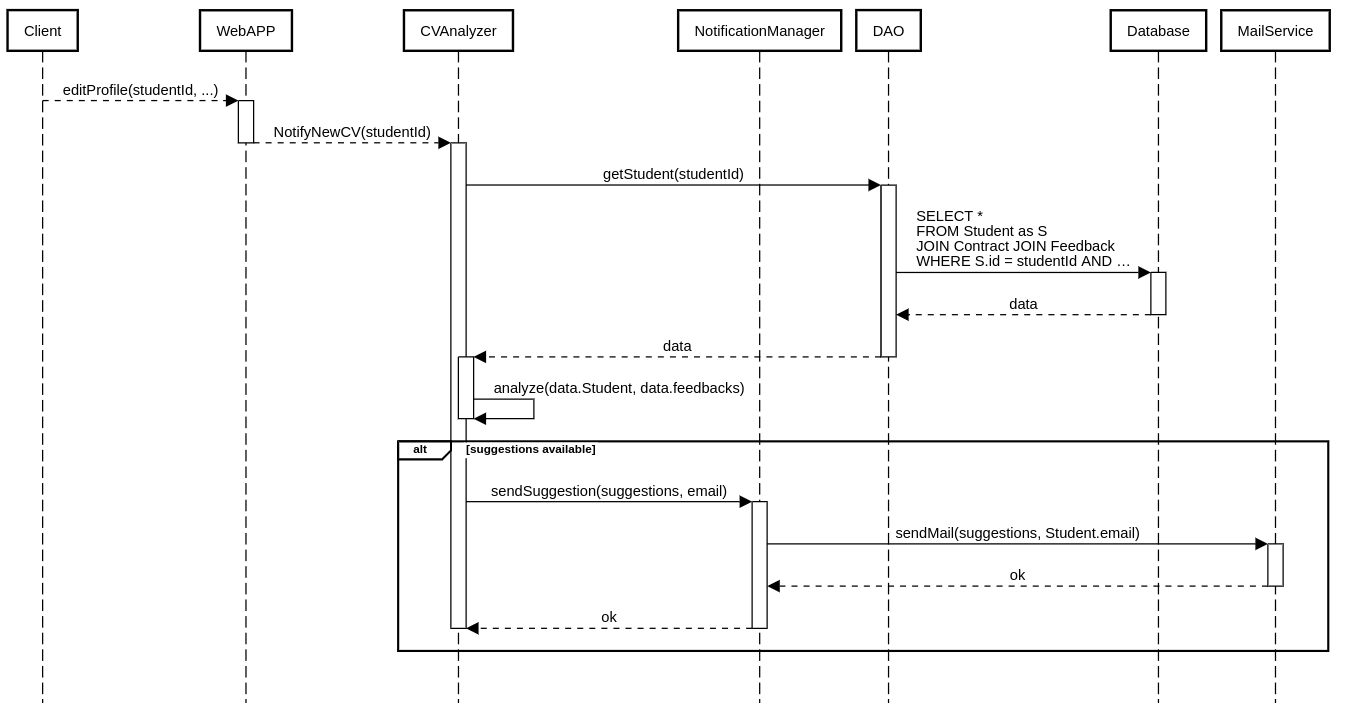
\includegraphics[width=\textwidth]{Images/UC diagrams/cv_suggestion.png}\newpage
[UC16] - Generate Internship Improvement Suggestion\newline
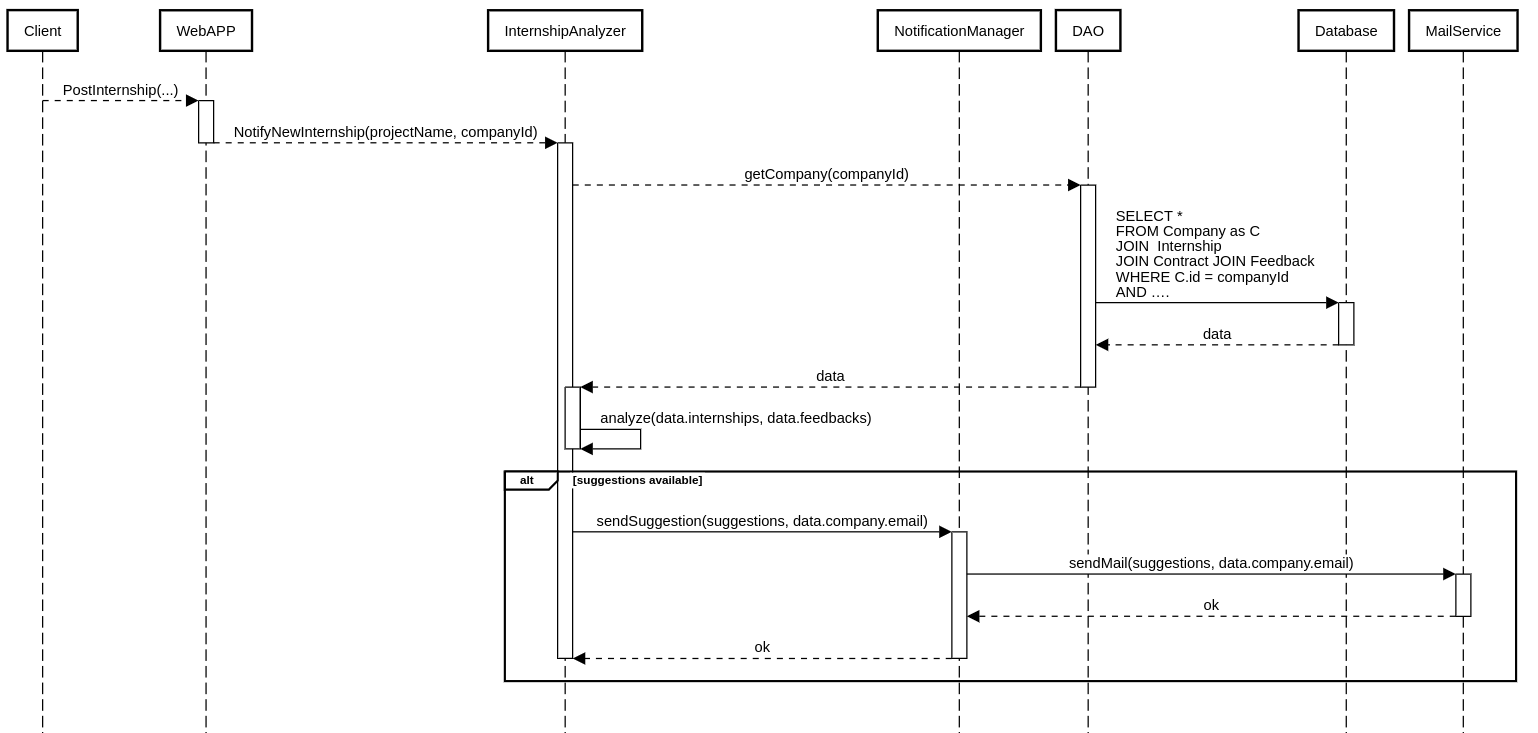
\includegraphics[width=\textwidth]{Images/UC diagrams/internship_suggestion.png}\newline
[UC17] - Student Recommendation\newline
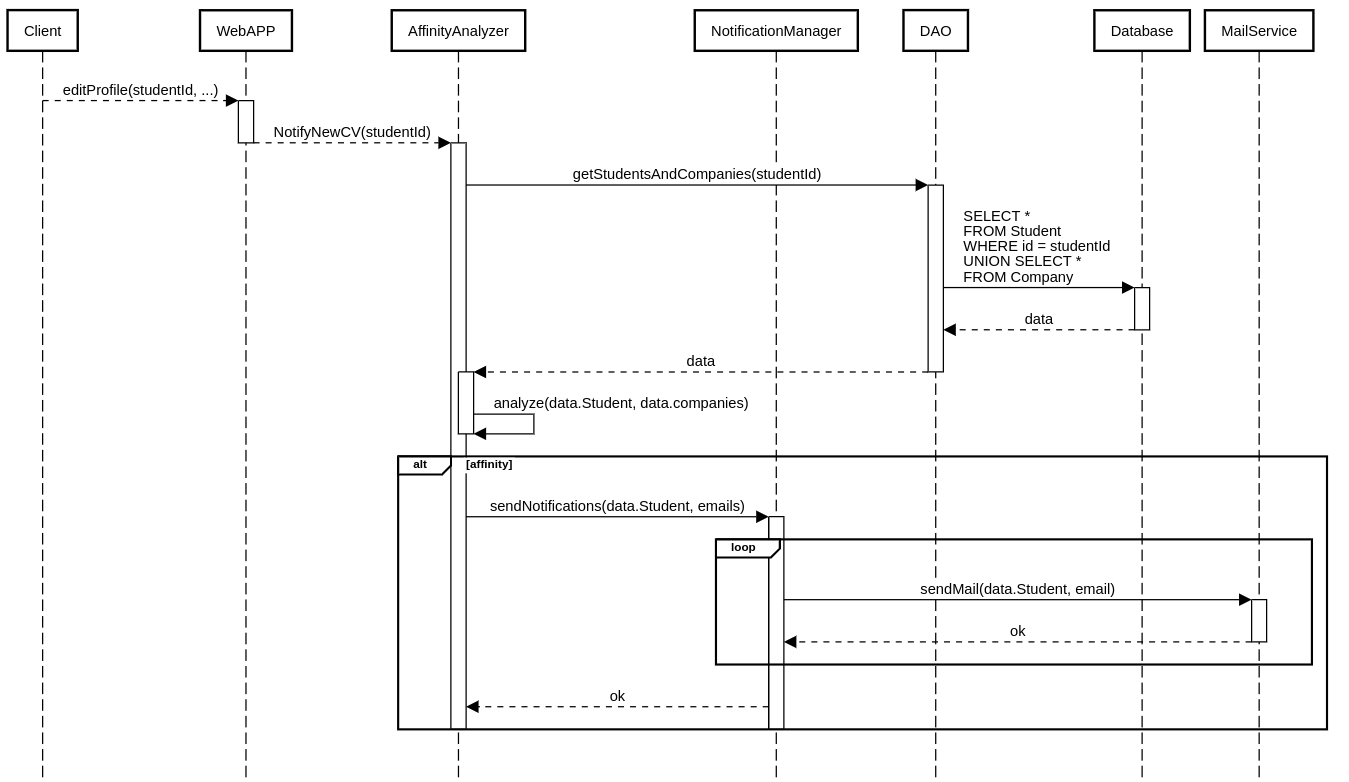
\includegraphics[width=\textwidth]{Images/UC diagrams/student_recommendation.png}\newpage
[UC18] - Internship Recommendation\newline
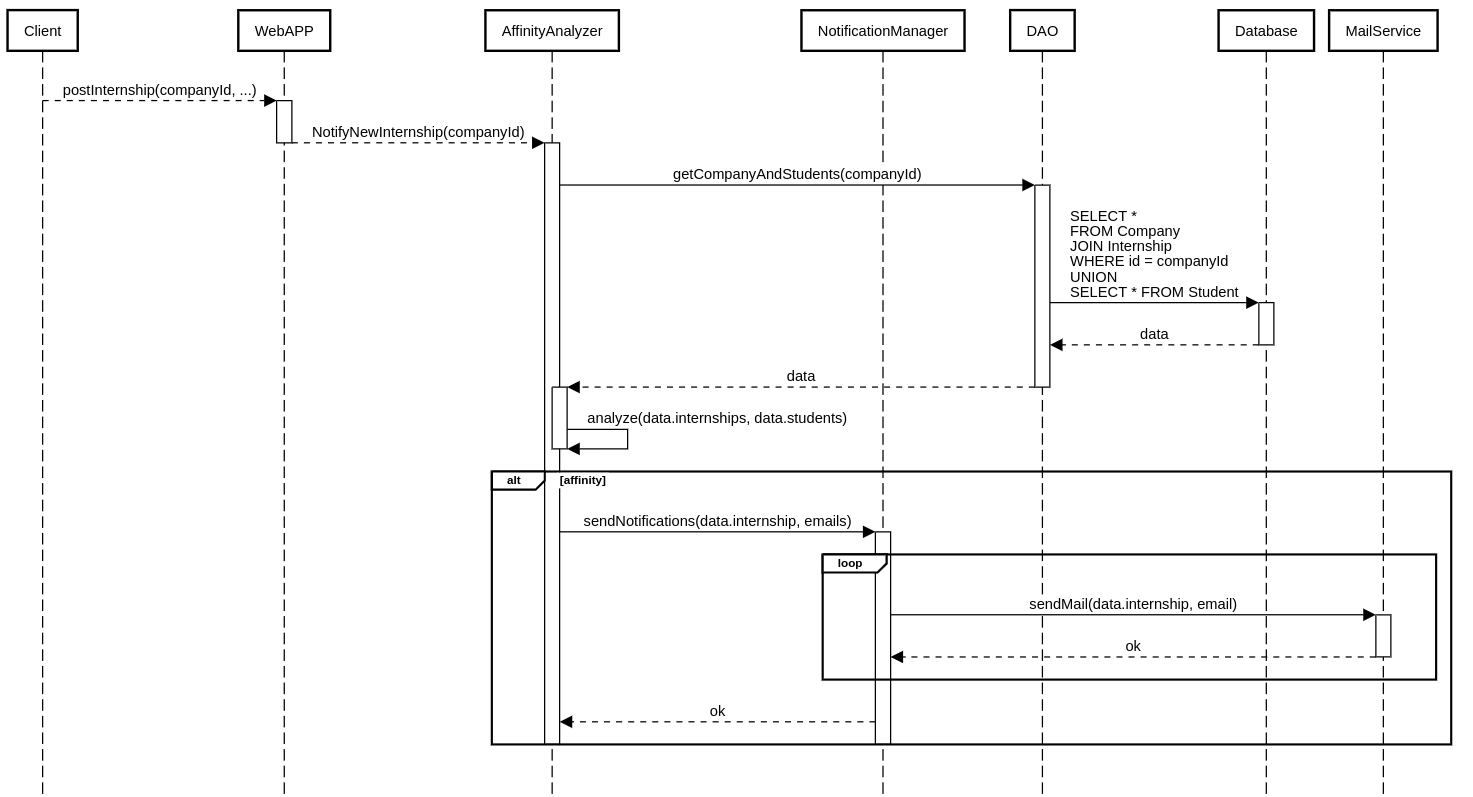
\includegraphics[width=\textwidth]{Images/UC diagrams/internship_recommendation.png}\newline
[UC19] - Monitor Internship Status\newline
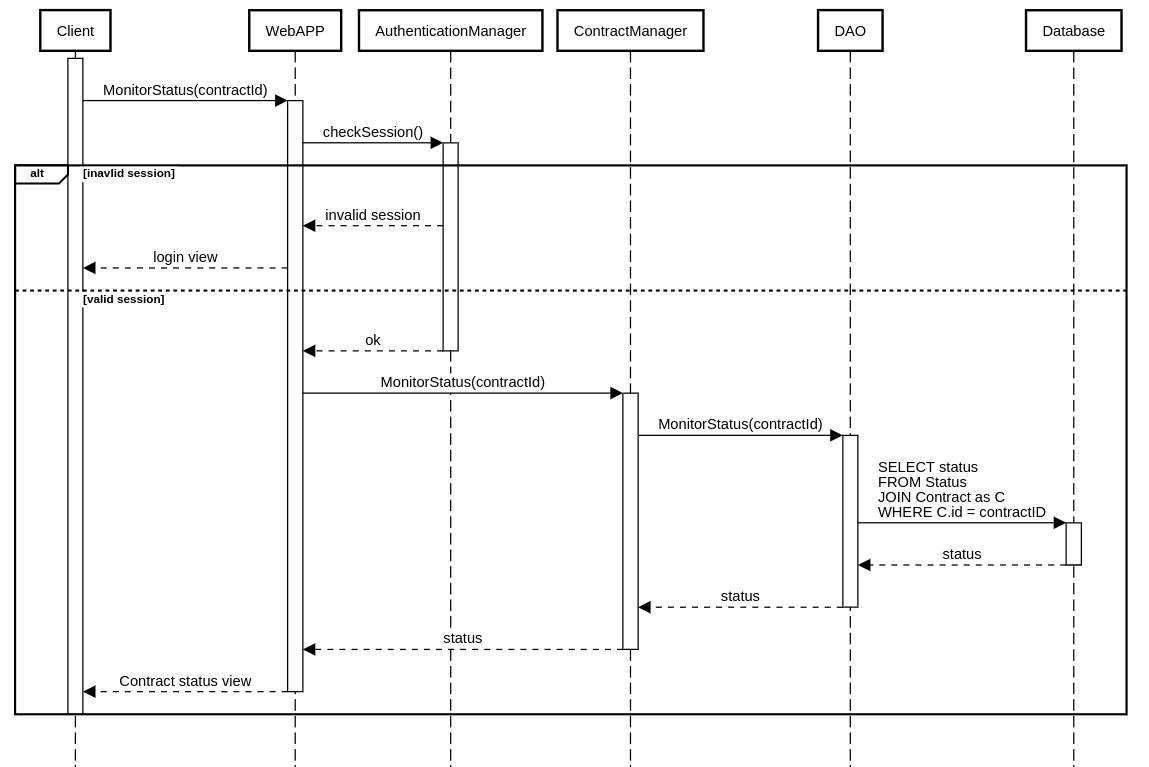
\includegraphics[width=\textwidth]{Images/UC diagrams/monitor_status.png}\newpage
[UC20] - Edit Profile\newline
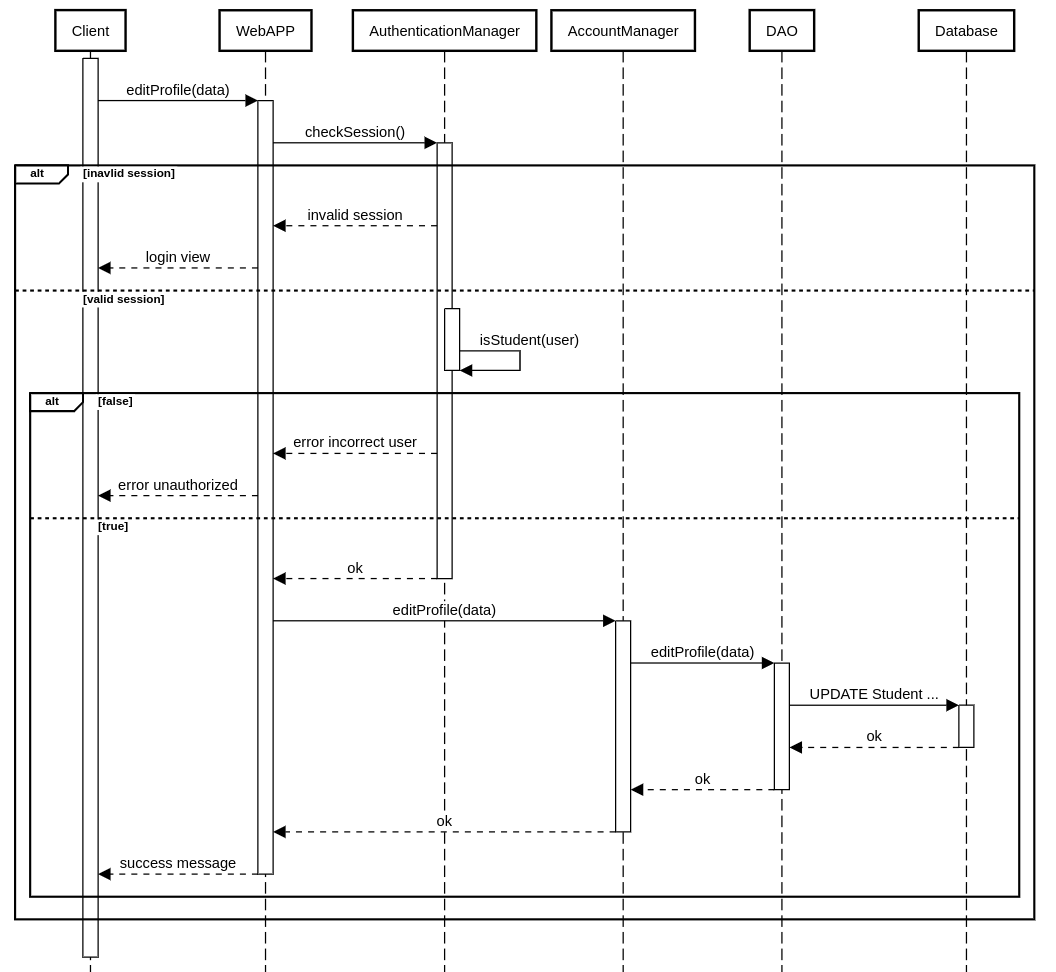
\includegraphics[width=\textwidth]{Images/UC diagrams/edit_profile.png}\newline









\subsection{Component Interfaces}
\subsubsection{WebAPP}
\begin{itemize}
    \item void: companyRegister.onClick()
    \item void: companyRegister(name, email, password, VAT)
    \item void: companyLogin.onClick()
    \item void: companyLogin(username, password)
    \item void: universityLogin.onClick()
    \item void: universityLogin(email, password)
    \item void: studentLogin.onClick()
    \item void: studentLogin(email, password)
    \item void: postInternship(projectName, description, termsConditions)
    \item void: postFeedback(rating, comment, contractId, userId)
    \item void: searchInternship(Options)
    \item void: apply(userId, internshipId)
    \item void: createQuestionnaire()
    \item void: answerQuestionnaire(contract, answers)
    \item void: signContract(userId, internshipId)
    \item void: openDiscussion(userId, internshipId, title, description)
    \item void: sendMessage(discussionId, content, userId)
    \item void: terminateContract(contractId)
    \item void: createQuestionnaire()
    \item void: monitorStatus(contractId)
\end{itemize}
\subsubsection{SheerID}
\begin{itemize}
    \item bool: SheerLogin(email, password)
\end{itemize}
\subsubsection{Database}
\begin{itemize}
    \item SELECT ...
    \item INSERT ...
    \item UPDATE ...
\end{itemize}
\subsubsection{DAO}
\begin{itemize}
    \item bool: isNewCompany(VAT)
    \item bool: isEndedContract(contractId)
    \item bool: isExistingFeedback(contractId, userId)
    \item bool: isExistingDiscussion(discussionId)
    \item bool: isAcceptedContract(userId, internshipId)
    \item bool: isExistingContract(contract, answers)
    \item bool: companyRegister(name, email, password, VAT)
    \item bool: companyLogin(username, password)
    \item bool: universityLogin(email, password)
    \item Student: getStudent(email)
    \item bool: createStudent(email, password)
    \item bool: postInternship(projectName, description, termsConditions)
    \item bool: postFeedback(rating, comment, contractId, userId)
    \item List<Internship>: SearchInternship(Options)
    \item bool: apply(userId, internshipId)
    \item bool: createQuestionnaire()
    \item bool: answerQuestionnaire(contract, answers)
    \item bool: signContract(userId, internshipId)
    \item bool: openDiscussion(userId, internshipId, title, description)
    \item bool: sendMessage(discussionId, content, userId)
    \item bool: terminateContract(contractId)
    \item bool: editProfile(data)
    \item bool: addQuestionnaire(questionnaire)
    \item STATUS: monitorStatus(contractId)
\end{itemize}
\subsubsection{AuthenticationManager}
\begin{itemize}
    \item JSON: createSession()
    \item bool: checkSession()
    \item Company: companyLogin(email, password)
    \item University: universityLogin(email, password)
    \item Student: studentLogin(email, password)
    \item bool: isCompany(user)
    \item bool: isStudent(user)
    \item bool: isUniversity(user)
\end{itemize}
\subsubsection{AccountManager}
\begin{itemize}
    \item bool: companyRegister(name, email, password, VAT)
    \item bool: editProfile(data)
\end{itemize}
\subsubsection{InternshipManager}
\begin{itemize}
    \item bool: postInternship(projectName, description, termsConditions)
    \item List<Internship>: SearchInternship(Options)
\end{itemize}
\subsubsection{ContractManager}
\begin{itemize}
    \item bool: apply(userId, internshipId)
    \item bool: addQuestionnaire(questionnaire)
    \item bool: signContract(userId, internshipId)
    \item bool: terminateContract(contractId)
    \item STATUS: MonitorStatus(contractId)
\end{itemize}
\subsubsection{FeedbackManager}
\begin{itemize}
    \item bool: postFeedback(rating, comment, contractId, userId)
\end{itemize}
\subsubsection{DiscussionManager}
\begin{itemize}
    \item bool: openDiscussion(userId, internshipId, title, description)
    \item bool: sendMessage(discussionId, content, userId)
\end{itemize}
\subsubsection{InterviewManager}
\begin{itemize}
    \item bool: answerQuestionnaire(contract, answers)
\end{itemize}
\subsubsection{InternshipAnalyzer}
\begin{itemize}
    \item void: NotifyNewIntership(projectName, companyId)
    \item {bool, String, email}: analyze(internship, feedbacks)
\end{itemize}
\subsubsection{CVAnalyzer}
\begin{itemize}
    \item void: NotifyNewCV(studentId)
    \item {bool, String, email}: analyze(student, feedbacks)
\end{itemize}
\subsubsection{AffinityAnalyzer}
\begin{itemize}
    \item {bool, String, List<email>}: analyze(student, companies)
    \item {bool, String, List<email>}: analyze(internship, students)
\end{itemize}
\subsubsection{NotificationManager}
\begin{itemize}
    \item bool: sendSuggestio(suggestions, email)
    \item bool: sendNotification(data, email)
\end{itemize}
\subsubsection{MailService}
\begin{itemize}
    \item bool: sendMail(data, mail)
\end{itemize}

\subsection{Selected Architectural Styles and Patterns}
\subsubsection{3-tier Architecture}
The architecture chosen for the S\&C system is a 3-tier client-server model, with the tiers assigned to the presentation, logic, and data layers, respectively. This architecture, characterized by highly decoupled components, enables the creation of a system that is both easily maintainable and flexible, allowing different aspects to be tested and updated independently. The tiers are described in more detail below:
\begin{itemize}
    \item \textbf{Web Client}: This tier is represented by web browsers, which provide the user interface for interacting with the system.
    \item \textbf{Application Server}: This tier handles all business logic, processes requests from the web client, and generates the pages or responses to be displayed on the clients.
    \item \textbf{Database Server}: This layer is simply a database for storing persistently and providing data as needed.
\end{itemize}
\subsubsection{Model View Controller Patter}
The Model-View-Controller (MVC) pattern is a widely used architectural design that aligns closely with the principles of the 3-tier architecture. In the MVC pattern, the Model represents the underlying data and business logic, corresponding to the database server and the DAOs of the application server. The View represents the user interface, similar to the web client tier, and is responsible for presenting data to the user. Finally, the Controller, implemented using the Handlers shown above, serves as the intermediary, handling user input and updating the Model or View as necessary. This separation of concerns allows for modular design, facilitating maintainability, scalability, and ease of testing, making the MVC pattern a natural fit for modern web and software applications.
\subsubsection{RESTful API}
The communication between client and server is handled through a REST API. This way, queries are HTTP based and can have an additional level of security using SSL encryption with HTTPS. Moreover REST has caching capabilities, enhancing performance even at scale since requests can be resolved directly by the client. Another advantage over other communication styles is statelessness which leads to naturally independent requests that can be handled concurrently.
\subsection{Other Design Decisions}
\subsubsection{Load Balancer}
A fundamental component in the system’s architecture is the load balancer. This device distributes incoming requests between the replicated application servers to avoid overloads resulting in increased response times and to seamlessly add (or remove) servers as needed. Load balancers can also protect the system from DDOS attacks, rate limiting clients issuing requests too frequently.